\documentclass[a4paper]{book}

\usepackage{amsmath,longtable,fancyhdr,booktabs,multirow,graphicx,float, bm}
\usepackage{amssymb}
\usepackage{color}
\usepackage[colorlinks,
            linkcolor=black,
            anchorcolor=blue,
            citecolor=green
           ]{hyperref}
\usepackage[top=1in,bottom=1in,left=1.25in,right=1.25in]{geometry}
\usepackage{CJKnumb,titlesec,titletoc}
\usepackage{mnsymbol}
\usepackage{theorem}
\usepackage{algorithmicx}
\usepackage{ulem}

\usepackage[nottoc]{tocbibind}
\def\ci{\perp\!\!\!\perp}
\pagestyle{fancy}
%% define some commands
\newcommand{\normD}{\mathcal{N}}
\newcommand{\mrm}{\mathrm}
\newcommand{\mbf}{\mathbf}
\newcommand{\mcal}{\mathcal}

\newcommand{\e}{\varepsilon}
\newcommand{\up}{\mathrm}
\def\dbar{\mathrm{\mathchar'26\mkern-12mu d}}
\newcommand{\wave}{\scriptsize{\sim}}
\newcommand{\bb}{\mathbb}
\newcommand{\mbb}{\mathbb}
\newcommand{\imp}[1]{\textit{#1}}
\newcommand{\bs}{\boldsymbol}
\newcommand{\mbs}{\boldsymbol}

\newcommand{\ud}{\mathrm{d}}
\newcommand{\mx}{\mrm x}
\newcommand{\mw}{\mrm w}
\newcommand{\md}{\mrm d}
\newcommand{\mB}{\mrm B}
\newcommand{\mW}{\mrm W}

\newcommand{\TT}{\mbf T}
\newcommand{\UU}{\mbf U}
\newcommand{\VV}{\mbf V}
\newcommand{\XX}{\mbf X}
\newcommand{\ZZ}{\mbf Z}
\newcommand{\WW}{\mbf W}
\newcommand{\RR}{\mbf R}
\newcommand{\MM}{\mbf M}
\newcommand{\KK}{\mbf K}
\newcommand{\II}{\mbf I}
\newcommand{\CC}{\mbf C}

\newcommand{\kk}{\mbf k}
\newcommand{\ww}{\mbf w}
\newcommand{\mm}{\mbf m}
\newcommand{\ttt}{\mbf t}
\newcommand{\bbb}{\mbf b}
\newcommand{\uu}{\mbf u}
\newcommand{\vv}{\mbf v}
\newcommand{\xx}{\mbf x}
\newcommand{\yy}{\mbf y}
\newcommand{\zz}{\mbf z}
\newcommand{\bmu}{\bm{\mu}}
\newcommand{\bphi}{\bm{\phi}}
\newcommand{\bmz}{\bm{0}}

\newcommand{\Exp}{\mathbb{E}}
\newcommand{\rev}{^{-1}}
\newcommand{\calD}{\mcal D}
\newcommand{\data}{\mcal D}
\newcommand{\cat}{\mcal C}
\newcommand{\trans}{^{\mrm T}}
\newcommand{\tit}{\textit}

\DeclareMathOperator*{\argmin}{arg\,min}
\DeclareMathOperator*{\argmax}{arg\,max}
\def\dbar{\mathrm{\mathchar'26\mkern-12mu d}}
\newcommand{\norm}[1]{\left\lVert#1\right\rVert}

\newtheorem{problem}{Problem}
\newtheorem{lemma}{Lemma}
\newtheorem{theorem}{Theorem}
\newtheorem{corollary}{Corollary}
\newtheorem{remark}{Remark}
\newtheorem{observation}{Observation}
\newtheorem{proposition}{Proposition}
\newtheorem{assumption}{Assumption}

\newcommand{\figref}[1]{Fig\onedot~\ref{#1}}
\newcommand{\equref}[1]{Eq\onedot~\eqref{#1}}
\newcommand{\secref}[1]{Sec\onedot~\ref{#1}}
\newcommand{\tabref}[1]{Tab\onedot~\ref{#1}}
\newcommand{\thmref}[1]{Thm\onedot~\ref{#1}}
\newcommand{\prgref}[1]{Program~\ref{#1}}
\newcommand{\clmref}[1]{Claim~\ref{#1}}
\newcommand{\lemref}[1]{Lemma~\ref{#1}}
\newcommand{\propref}[1]{Prop\onedot~\ref{#1}}
\newcommand{\ptyref}[1]{Property\onedot~\ref{#1}}
\newcommand{\yangs}[1]{{\color{cyan}{\bf\sf [YS: #1]}}}
\newcommand{\yang}[1]{{\color{cyan}{\bf\sf [#1]}}}
\newcommand{\Ep}{\mcal{E}}
\newcommand{\Epp}{\widehat{\mcal{E}}_s^+[\mu]}
\newcommand{\Eln}{\widehat{\mcal{E}}_{\lambda,n}[\mu]}
\newcommand{\mup}{\widehat{\mu}_{(X,Y)}^+}
\newcommand{\muln}{\widehat{\mu}_{\lambda,n}}
\newcommand{\Hy}{\mcal{H}_{\mcal{Y}}}
\newcommand{\Hx}{\mcal{H}_{\mcal{X}}}
\newcommand{\HK}{\mcal{H}_{K}}
\newcommand{\hC}{\widehat{\mcal{C}}}


\def\eg{\emph{e.g}\onedot}
\def\Eg{\emph{E.g}\onedot}
\def\ie{\emph{i.e}\onedot}
\def\Ie{\emph{I.e}\onedot}
\def\cf{\emph{cf}\onedot}
\def\Cf{\emph{Cf}\onedot}
\def\etc{\emph{etc}\onedot}
\def\vs{\emph{vs}\onedot}
\def\wrt{w.r.t\onedot}
\def\dof{d.o.f\onedot}
\def\aka{a.k.a\onedot}
\def\iid{i.i.d\onedot}
\def\etal{\emph{et al}\onedot}

\title{Notes of PRML}
\author{Siyu Wang}
\date{August 2018}

\begin{document}

\maketitle

\chapter{Mathematical Foundations}
\section{Probability Theory}
sum rule: $$p(X) = \sum_Yp(X,Y)$$
product rule: $$p(X,Y) = p(Y|X)p(X)$$
Question: what is the most different thing between bayesian and non-bayesian?
\subsection{probability densities}
continuous variables for $$x = g(y)$$ , $$p_y(y) = p_x(x)|\frac{dx}{dy}| = p_x(g(y))|g'(y)|$$
Bayes' theorem still applies to probability densities or combination of discrete and continuous variables:
$$p(x) = \int p(x, y)\mathrm{d}y$$
$$p(x,y) = p(y|x)p(x)$$
\subsection{Expectations and covariances}
\textit{variance} for one variable $f(x)$: $$\mathrm{var}[f] = E[(f(x)-E[f(x)])^2]$$
\emph{covariance} for two variables $x, y$: $$\mathrm{cov}[x,y]= E_{x,y}[\{x-E[x]\}\{y-E[y]\}]$$
for two vectors of random variables $\textbf{x}$ and $\textbf{y}$, the covariance is a matrix
$$\mathrm{cov}[\textbf{x}, \textbf{y}] =E_{x,y}[\{\textbf{x}-E[\textbf{x} ]\}\{\textbf {y}^T-E[\textbf {y}^T]\}]$$
and for one vector $$\mathrm{cov}[\textbf{x}] = \mathrm{cov}[\textbf {x},\textbf {x}]$$
\subsection{Bayesian probabilities}
essential idea: convert a prior probability into a posterior proboability.
\begin{equation}\label{eq1.1}
  p(\textbf{w},\mathcal{D}) = \frac{p(\mathcal{D}|\textbf {w})p(\textbf {w})}{p(\mathcal{D})}
\end{equation}
note that\newline
$p(\textbf w)$: before observing the data, in the form of a prior probability distribution\newline
$\mathcal{D}$ : observed data $\{t_1,\dots, t_n\}$\newline
$p(\mathcal{D})$ : seen as a normalization constant.\newline
$p(\mathcal{D}|\textbf w)$ : \emph{likelihood function}.  a function of the parameter vector $\textbf w$ , expresses how probable the observed data set is for different settings of the parameter vector $\textbf  w$
key idea can be sumed as:
\begin{equation}\label{eq1.2}
\mathrm{posterior} \propto \mathrm{likelihood} \times \mathrm{prior}
\end{equation}
\textbf{Bayesian and frequentist paradigm}
for frequentist, $\textbf  w$ is considered to be fixed parameter and its vlaue is determined by some form of 'estimator'.\newline
one common frequentist estimator is \emph{maximum likelihood},  maximize likelihood function $p(\mathcal{D}|\textbf w)$, in machine learning, negative lof og the likelihood function is called an \emph{error function}.\newline
\emph{bootstrap} technique.\newline
for Bayesian, there is only a single data set $\mathcal{D}$ and the uncertainty in the parameters is expressed through a probability distribution over $\textbf w$\newline
inclusion of prior knowledge\newline
how to select prior distribution is a problem for Bayesian method.\newline
Reducing the dependence on the prior. \emph{noninformative} priors
\subsection{The Gaussian distribution}
For one variable:
\begin{equation}\label{eq1.3}
  \mathcal{N}(x|\mu,\sigma^2) = \frac{1}{(2\pi\sigma^2)^{1/2}}\exp\{-\frac1{2\sigma^2}(x-\mu)^2\}
\end{equation}
for D-dimensional vector:
\begin{equation}\label{eq1.4}
  \mathcal{N}(\textbf x|\mu, \Sigma) = \frac{1}{(2\pi)^{D/2}}\frac1{|\Sigma|^{1/2}}\exp\{-\frac12(\textbf x-\mu)^T\Sigma^{-1}(\textbf x-\mu)\}
\end{equation}
Problem : observations for N times $\textbf x=(x_1,\dots,x_N)^T$,  we want to get parameters for the Gaussian distribution.
Then the likelihood function$p(\mathcal{D}|\textbf w)$ is just $p(\textbf x|\mu, \sigma^2) = \Pi_{n=1}^{N}\mathcal{N}(x_n|\mu,\sigma^2)$.
so using ML criterion, we will want to maximize $\ln p(\textbf x|\mu,\sigma^2)$ and we can get
$$\mu_{ML} = \frac1N\sum_{n=1}^Nx_n, \mathrm{sample mean}$$,
$$\sigma_{ML}^2 = \frac1N\sum_{n=1}^N(x_n-\mu_{ML})^2, \mathrm{sample variance}$$
but we can infer that:
$$E[\mu_{ML}] = \mu$$
$$E[\sigma_{ML}^2] = (\frac{N-1}N)\sigma^2$$ rather than exactly $\sigma^2$
this can be inferred from inspiration in figure\ref{fig1.1}:
\begin{figure}
  \centering
  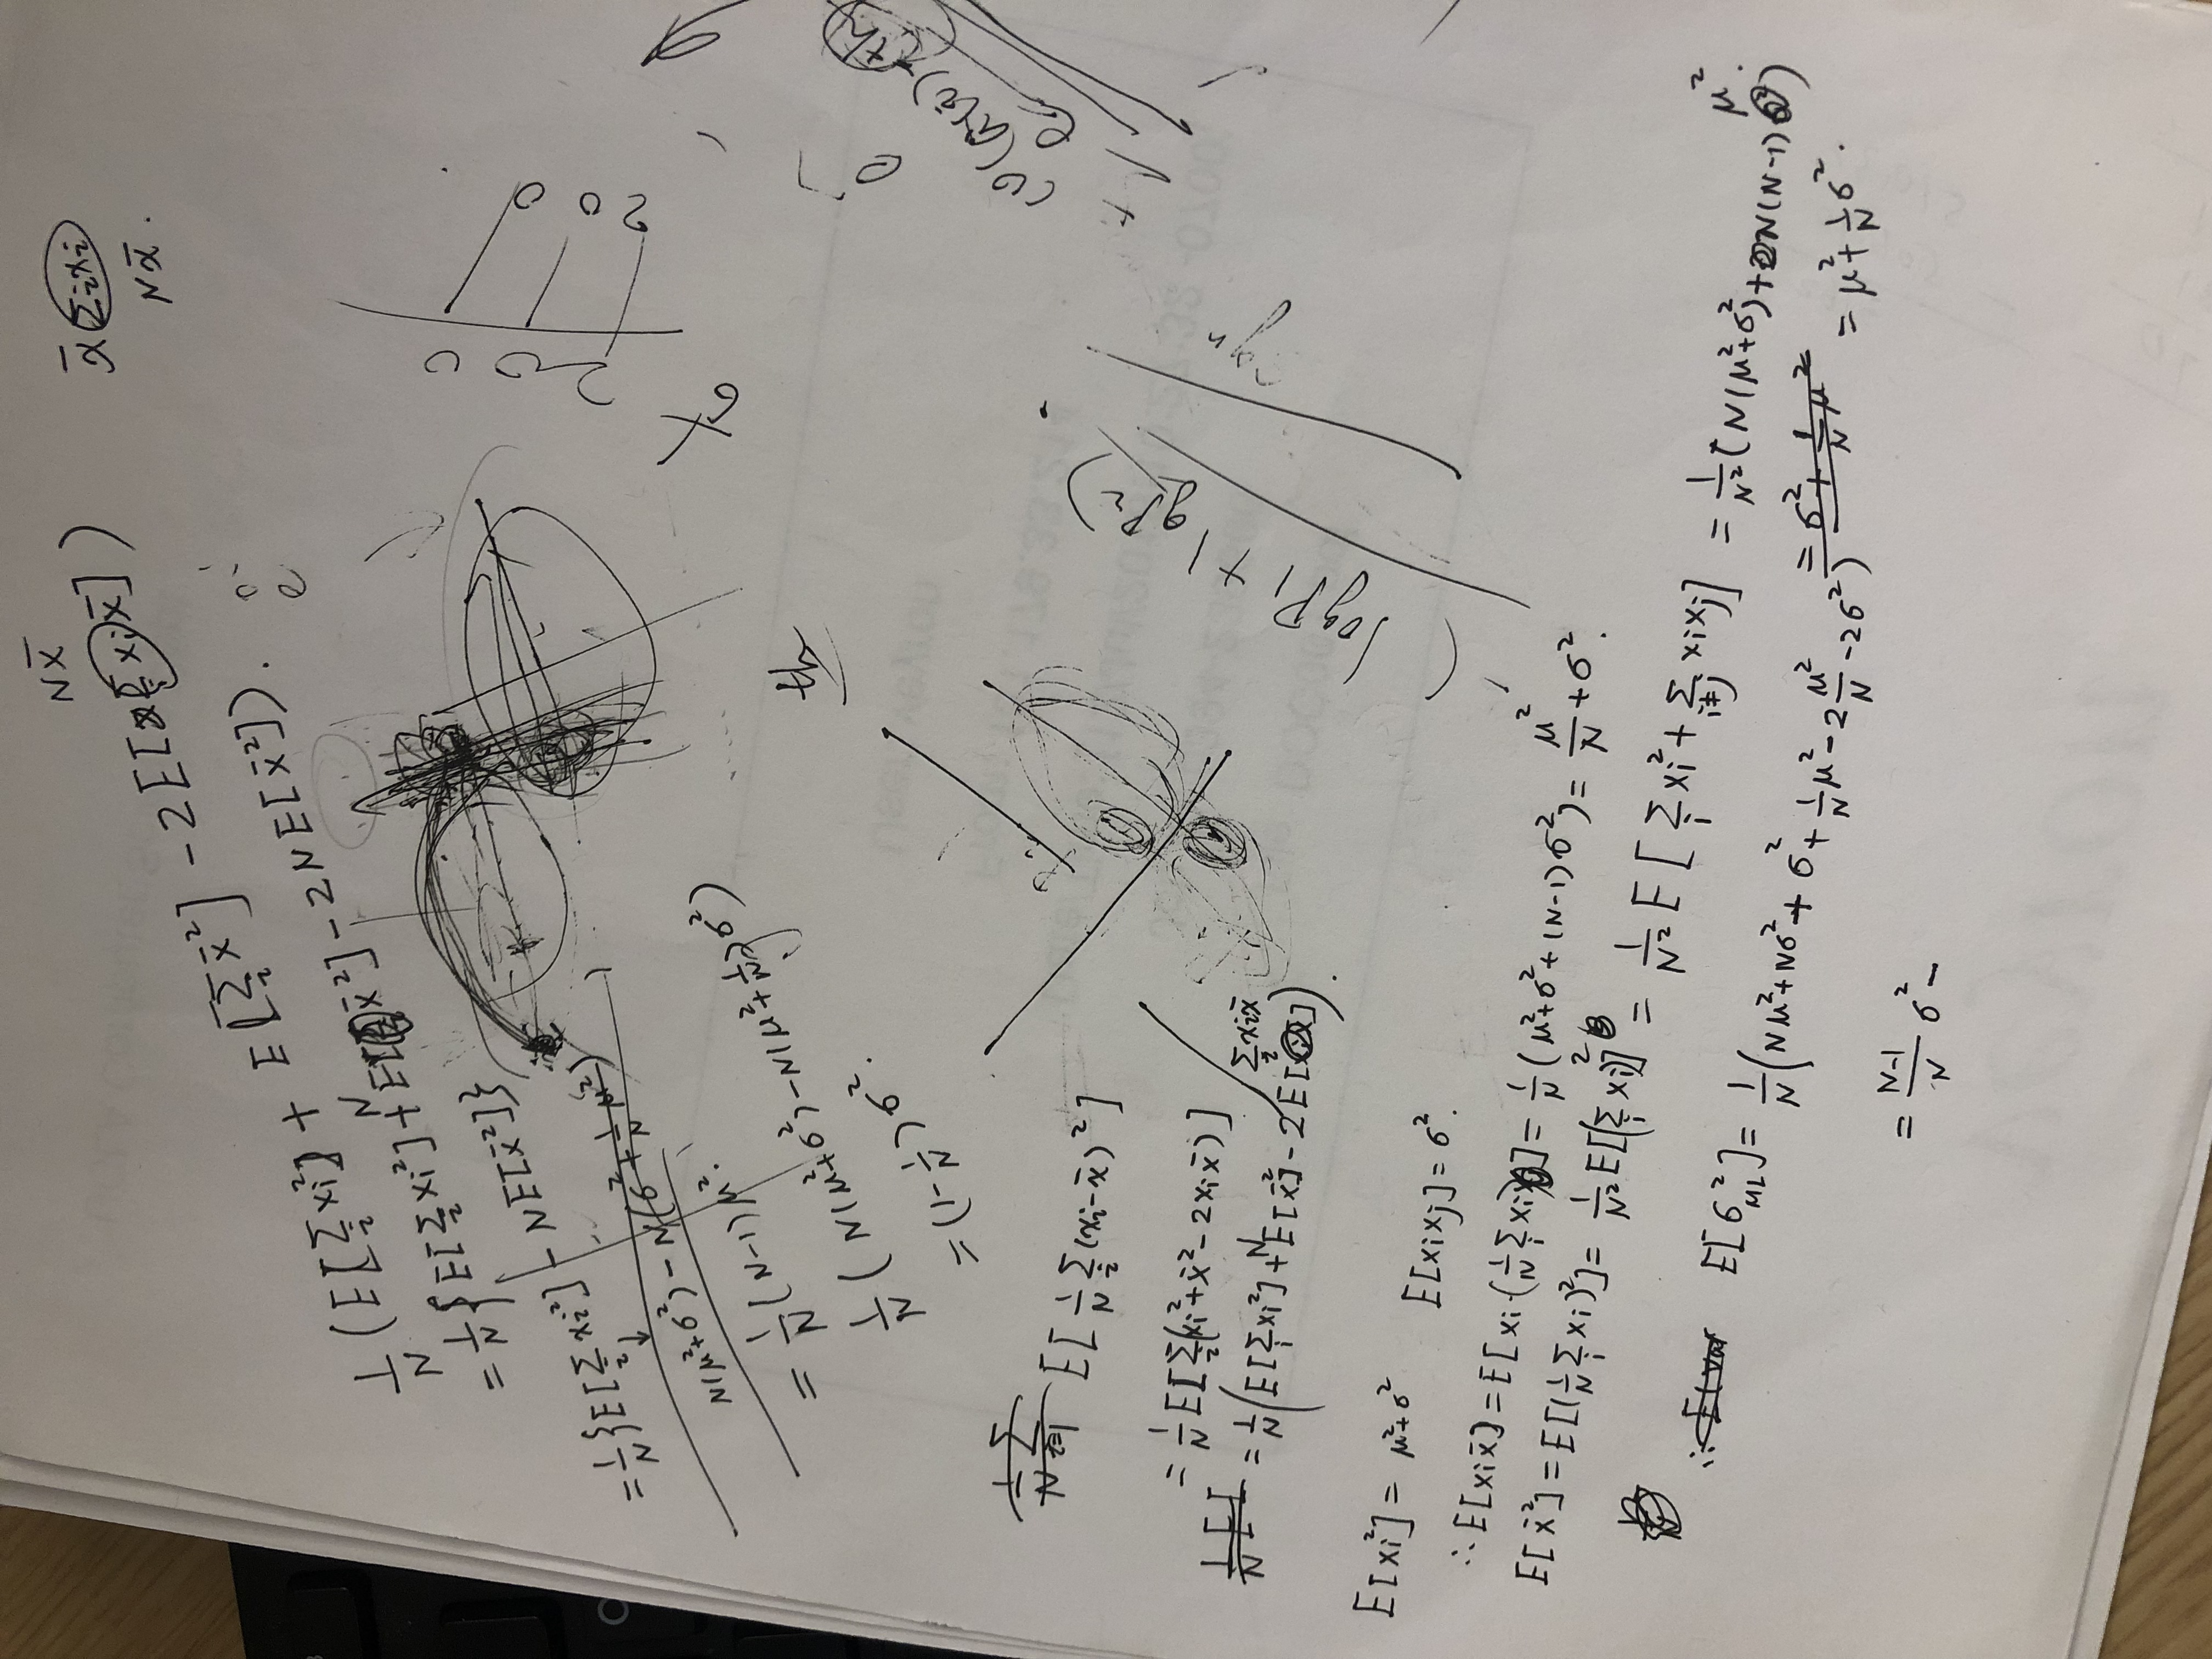
\includegraphics[width=\linewidth]{./imgs/infer1.jpg}
  \caption{Inference}\label{fig1.1}
\end{figure}
but there seems to be more convenient way using chi-sqaure distribution
\subsection{Curve fitting re-visited}
This time, we model curve fitting problem by : given the value of $x$, the corresponding value of $t$ has a Gaussian distribution with a mean equal to the value $y(x,\textbf w)$ (polynomial curve).
\begin{equation}\label{eq1.9}
  p(t|x,\textbf w,\beta) = \mathcal{N}(t|y(x,\textbf w),\beta^{-1})
\end{equation}
\begin{equation}\label{eq1.10}
  p(\textbf t|\textbf x,\mathrm{w},\beta) = \Pi_{n=1}^N\mathcal N(t_n|y(x_n,\mathrm{w}),\beta^{-1})
\end{equation}
and log likelihood function can be derived from above.  and\textbf{
Maximizing likelihood is equivalent to minimizing the sum-of-squares \emph{error function} defined earlier !!!}\newline
if we use Bayesian method and assume prior distribution over \textbf{w}:
\begin{equation}\label{eq1.5}
  p(\mathrm{w}|\alpha) = \mathcal{N}(\mathrm{w}|\textbf{0},\alpha^{-1}\textbf I) )
\end{equation}
$\alpha$ is called \emph{hyperparameters}. Using Bayesian rules to get
\begin{equation}\label{eq1.6}
  p(\mathrm w|\textbf{x}, \textbf t, \alpha,\beta) \propto p(\textbf t|\textbf x,\mathrm w,\beta)p(\mathrm w|\alpha)
\end{equation}
Using \emph{maximizing the posterior distribution, MAP} and we find the maximum of the posterior is given by the minimum of:
\begin{equation}\label{eq1.7}
 \frac{\beta}2\sum_{n=1}^N\{y(x_n,\mathrm{w})-t_n^2+\}\frac{\alpha}2\mathrm{w}^T\mathrm{w}
\end{equation}
so this is similar to regularize sum-od-squares error function with $\lambda=\frac{\alpha}{\beta}$
\subsection{Decision Theory}
\textbf{minimizing the misclassification rate} $p(\mathrm{mistake})$ and $p(\mathrm{correct})$ \newline
\textbf{minimizing the expected loss}\newline
can assign different loss efficient to different error
\begin{equation}\label{eq1.8}
  E[L] = \sum_k\sum_j\int_{\mathcal{R}_j}L_{kj}p(\mathrm{x},\mathcal{C}_k)\mathrm {dx}
\end{equation}
$p(\mathrm{x},\mathcal{C}_k) = p(\mathcal{C}_k|\mathrm{x})p(\mathrm{x})$ to eliminate the common factor $p(\mathrm x)$ \newline
\textbf{ inference and decision}\newline
Three distinct approaches:
\begin{enumerate}
    \item First solve $p(\mrm{x}|\mathcal C_k)$ as well as $p(\mathcal C_k$ for each class individually, then figure out $p(\mathcal C_k|\mrm x) = \frac{p(\mathrm x|\mathcal C_k)p(\mathcal C_k)}{p(\mrm x)}$ and $p(\mrm x)$ can be gotten from $p(\mrm x) = \sum_kp(\mrm x|\mathcal C_k)p(\mathcal C_k)$. This is equivalent to model the joint distribution $p(\mrm x, \mathcal C_k)$
  \item Determine posterior class probabilities $p(\mathcal C_k|\mrm x)$  and then use decision theory.  \emph{discriminative model}.
  \item Find $f(\mathrm x)$ which maps $\mrm{x}$ directly to a class label.
\end{enumerate}
The first approach is too time-consuming and demanding, while the last one is simplest but not so robust as approach.2 because we can see a lot of information from the posterior probabilities:
\begin{itemize}
  \item  minimizing risk,  by adjusting $L_{kj}$ to get different loss function and minimize risk
  \item reject option
  \item \textbf{compensating for class priors} \uline{this is not thought of by myself but very important. sometimes we have to make training set more suitable for learning features, but this operation on training set will lead to a modification on prior probabilities so we must revise this part by divide by the class fraction in the data set and then multiply by the class fraction in the population of which we want to apply this model.}
  \item combining models.
\end{itemize}
\textbf{Loss function for regression}
$$E[L] = \iint L(t,y(\mathrm x))p(\mathrm  x,t)\mathrm {dx}$$
If we define
\begin{equation}\label{eq1.11}
  L(t,y(\mathrm  x)) = \{y(\mathrm  x)-t\}^2
\end{equation}
we can get $y(\mathrm  x) = E_t[t|\mathrm  x]$ to minimize $E[L]$.\newline
Similarly, we also have three approaches using joint probability, posterior probability and a direct regression function $f(\mathrm  x)$\newline
sometimes we define $L$ by \emph{Minkowski} loss as $L_q = |y(\mathrm  x)-t|^q$
\subsection{Information Theory}
Look for a quantity $h(x)$ than is a monotonic function of the probability $p(x)$ and that expresses the information content. and should satisfy
$$h(x,y) = h(x)+h(y)$$.
so we define$$h(x) = -\log_2p(x) (bits)$$  or $$h(x) = -\ln p(x), nats$$
\textbf{ENTROPY}:
\begin{equation}\label{eq1.18}
  H[x] = E[h(x)]= -\sum_xp(x)\log_2p(x)
\end{equation}
relative to \emph{statistical physics}.\newline
To define entropy for continuous variable:\newline
differential entropy: $H[\mathrm x] = -\int p(\mathrm x)\ln p(\mathrm x)$

\textbf{maximizing entropy} by using Lagrange multipliers\newline
\begin{itemize}
  \item for discrete, uniform distribution
  \item  for continuous, Gaussion distribution $H[x] = \frac12[1+\ln (2\pi\sigma^2)]$
\end{itemize}
conditional entropy:
\begin{equation}\label{eq1.12}
H[y|x] = \iint p(y,x)\ln p(y|x) \mathrm dy\mathrm dx
\end{equation}
so  $H[x,y]=H[y|x]+H[x]$.
\subsubsection{Relative entropy and mutual information}
\textbf{KL divergence (relative entropy)}
\begin{equation}\label{eq1.13}
  \mathrm {KL}(p||q) = -\int p(x)\ln q(x)\mathrm dx-(-\int p(x)\ln p(x)\mathrm dx) = -\int p(x)\ln \frac{q(x)}{p(x)}
\end{equation}
this is not symmetrical!\newline
when we use \emph{convex} function and Jensen's unequality,
\begin{equation}\label{eq1.14}
  f(\int xp(x)\mathrm  dx) \leq \int f(x)p(x) \mathrm dx
\end{equation}
also as $f(E[x]) \le E[f(x)]$ we can get
\begin{equation}\label{eq1.14}
  \mathrm  {KL}(p||q) = -\int p(x)\ln\{\frac{q(x)}{p(x)}\}\mathrm  dx \ge -\ln\int q(x)\mathrm  dx = 0
\end{equation}
\uline{BUT I think here, in order to get unequality for KL-divergence , Jensen's unequality should be generalized to $f(E[k(x)])\le E[f(k(x))]$, to be more precise}
the most important thing is , KL divergence can be used as a measure of the dissimilarity of two distributions $p(x)$ and $q(x)$
\subsubsection{to approximate an unknown distribution p(x)}
we have observed a finite set of training points $\mathrm x_n$ for $n=1,2,\dots,N$ drawn from $p(\mathrm  x)$
here we must pay attention that we are not getting points from the distribution curve, we are getting points distributed as $p(\mathrm  x)$ says.
So
\begin{equation}\label{eq1.15}
  \mathrm {KL}(p||q) = -\mathrm  E[\ln\frac{q(\mathrm x)}{p(\mathrm x)}]\simeq\sum_{n=1}^N\{-\ln q(\mathrm  x_n|\theta) +\ln p(\mathrm x_n)\}
\end{equation}
\subsubsection{consider joint distrbiution between two sets of variables x and y}
$p(x,y) = p(x)p(y)$ if x and y is independent.
When they are dependent, we want to use KL divergence between joint distribution and the product of marginals to see how close they are  to independent.
\begin{equation}\label{eq1.16}
  I[x,y] = \mathrm {KL}(p(x,y)||p(x)p(y)) = -\int\int p(x,y)\ln(\frac{p(x)p(y)}{p(x,y)})
\end{equation}
this is \emph{mutual information} between x and y  and
\begin{equation}\label{eq1.17}
I[x,y] = H[x]-H[x|y]
\end{equation}
The mutual information represents the reduction in uncertainty about x as a consequence of the new observation y.
\subsection{Some other distributions}
\subsubsection{Poisson distribution}
\subsubsection{Laplace dsitribution}

\subsection{Conclusion}
The most important thought in this chapter is difference between Bayesian and non Bayesian,, e.g. ML and MAP.  Sometimes ML is equivalent to minimizing error function and MAP can be equivalent to them, too.\newline
The most important thing stepping from non Bayesian to Bayesian, is the inclusion of prior probability and we use $$\mathrm{posterior} \propto \mathrm{likelihood} \times\mathrm{prior}$$
To see this problem from angel of information theory, we can find KL divergence between $p(x,y)$ and $p(x)p(y)$ will be mutual information between x and y. And this represent the reduction in uncertainty about x as a consequence of the new observation y.

\section{Probability Distributions}
In the frequentist treatment , we choose specific values for the parameters by optimizing some criterion, such as the likelihood function. But, in a Bayesian treatment we introduce prior distribution over the parameters and then use Bayes' theorem to compute the corresponding posterior distribution given the observed data.\newline
limitation:  assumes a specific functional form of the distribution.
\subsection{Binary Variables}
\begin{gather}\label{eq1.2.1}
  p(x=1|\mu) = \mu \\
  \mathrm {Bern}(x|\mu) = \mu^x(1-\mu)^{1-x} \\
  \mathrm E[x] = \mu, \mathrm  {var}[x]=\mu(1-\mu)
\end{gather}
data set $\mathcal D={x_1,\dots,x_N}$ of observed values of $x$, independently.\newline
then we can construct the likelihood function
\begin{equation}\label{1.2.2}
p(\mathcal D|\mu) = \Pi_{n=1}^Np(x_n|\mu) = \Pi_{n=1}^N\mu^{x_n}(1-\mu)^{1-x_n}
\end{equation}
log likelihood function $\ln p(\mathcal D|\mu)$\newline
maximize likelihood can lead to $\mu_{ML} = \frac1N\sum_{n=1}^Nx_n$ , and $\sum_{n=1}^Nx_n$ is called \emph{sufficient statistic}\newline
Denote the number of observation of $x = 1 $ within this data set by $m$, then  $\mu_{ML}=\frac mNN$. \newline
\uline{But,we can get extreme result using maximum likelihood criterion!}
\textbf{binomial distribution}
$$\mathrm{Bin}(m|N,\mu) = C_N^m\mu^m(1-\mu)^{N-m} $$
$$\mathrm E[m]=N\mu, \mathrm  {var}[m]=N\mu(1-\mu)$$
\subsubsection{The beta distribution}
we choose an appropriate prior  distribution so that the posterior distribution will have the same functional form as the prior. so \emph{beta distribution} comes.
\begin{gather}\label{1.2.3}
  \mathrm  {Beta}(\mu|a,b) = \frac{\Gamma(a+b)}{\Gamma(a)\Gamma(b)}\mu^{a-1}(1-\mu)^{b-1}
\Gamma(x)=\int_0^\infty u^{x-1}e^{-u}\mathrm du
\end{gather}
The distribution is normalized.
$$\mathrm E[\mu] = \frac a{a+b}, \mathrm {var}[\mu] = \frac{ab}{(a+b)^2(a+b+1)}$$
$a$ and $b$ are \emph{hyperparameters} controlling the distribution of the parameter $\mu$.\newline
so we can get posterior distribution:
$$p(\mu|m,l,a,b) \propto \mu^{m+a-1}(1-\mu)^{l+b-1}$$
and after normalization we get:
$$p(\mu|m,l,a,b) = \frac{\Gamma(m+a+l+b)}{\Gamma(m+a)\Gamma(l+b)} \mu^{m+a-1}(1-\mu)^{l+b-1}$$
The posterior can act as the prior if we subsequently observe additional data.
\emph{sequential approach}:
Sequential methods make use of observations one at a time, or in small batches, and then discard them before the next observations are used.\newline
and
\begin{equation}\label{1.2.4}
  p(x=1|\mathcal D) = \int_0^1p(x=1|\mu)p(\mu|\mathcal D)\mathrm d\mu = \int_0^1\mu p(\mu|\mathcal D)\mathrm d\mu=\mathrm E[\mu|\mathcal D]
\end{equation}
$=\frac{m+a}{m+a+l+b}$\newline
so when $m,l\rightarrow \infty$, it reduce to $\frac{m}{m+l}$\newline
when the number of observations increases, the posterior distribution becomes more sharply peaked, which can be seen from the variance.
\textbf{and this is a general property of Bayesian learning!}\newline
process of inferring can be seen at **page74** in the book.
\subsection{Multinomial Variables}
an extension to binary variables\newline
$\mathrm x = (x_1,\dots,x_K)^T$ one-hot\newline
denote, the probability of $x_k = 1$ by the parameter $\mu_k$ and $\sum_{k=1}^K\mu_k = 1$\newline
so, $p(\mathrm x|\mu) = \Pi_{k=1}^K\mu_k^{x_k}$\newline
data set $\mathcal D$ of $N$ independent observations $\mathrm x_1, \dots, \mathrm x_N$\newline
so likelihood function is:
\begin{equation}\label{1.2.5}
  p(\mathcal D|\mu) = \Pi_{n=1}^N\Pi_{k=1}^K\mu_k^{x_{nk}} = \Pi_{k=1}^K\mu_k^{\sum_nx_{nk}} = \Pi_{k=1}^K\mu_k^{m_k}
\end{equation}
where $m_k = \sum_nx_{nk}$ represents the number of observations of $x_k = 1$, \emph{sufficient statistics} for this distribution\newline
to do ML, maximize $\sum_{k=1}^Km_k\ln \mu_k+\lambda(\sum_{k=1}^K\mu_k-1)$ and we get $\mu_k^{ML} = \frac{m_k}{N}$
\begin{equation}\label{1.2.6}
  \mathrm {Mult}(m_1,\dots,m_K|\mu,N) = \left(\begin{matrix}N\\m_1m_2\dots m_K\end{matrix}\right)\Pi_{k=1}^K\mu_k^{m_k}
\end{equation}
\subsubsection{The Dirichlet distribution}
a family of prior distributions for the parameters $\{\mu_k\}$ of the multinomial distribution.
\begin{equation}\label{1.2.7}
  p(\mu|\alpha) = \frac{\Gamma(\alpha_0)}{\Gamma(\alpha_1)\dots\Gamma(\alpha_K)}\Pi_{k=1}^K\mu_k^{\alpha_k-1}
\end{equation}
 where $\alpha_0 = \sum_{k=1}^K\alpha_k$.
then posterior probability will be $p(\mu|\mathcal D, \alpha) = \mathrm {Dir}(\mu|\alpha+\mathrm m)$
\section{The Gaussian Distribution}
the sum of multiple random variables
\textbf{central limit theorem}
\begin{equation}\label{1.2.8}
  \mathcal N(\mathrm x|\mu, \Sigma) = \frac1{(2\pi)^{D/2}|\Sigma|^{1/2}}\exp\{-\frac12(\mathrm x-\mu)^T\Sigma^{-1}(\mathrm x-\mu)\}
\end{equation}
dependence on $\mathrm x$ is through a quadratic form:
$$\Delta^2 = (\mathrm x-\mu)^T\Sigma^{-1}(\mathrm x-\mu)$$ in the exponent.\newline
We can take $\Sigma$ to be symmetric because ant antisymmetric component would disappear from the exponent.
consider eigenvalues (real number because of $\Sigma$'s reality and symmetry) of $\Sigma$
\begin{equation}\label{1.2.9}
  \Sigma \mathrm u_i= \lambda_i\mathrm u_i, i = 1,2,\dots,D
\end{equation}
$\mathrm u_i^T\mathrm u_j = I_{ij}$

then $\Sigma = \sum_{i=1}^D\lambda_i\mathrm u_i\mathrm u_i^T$ and $\Sigma^{-1} = \sum_{i=1}^D\frac1{\lambda_i}\mathrm u_i\mathrm u_i^T$

and define $y_i=\mathrm u_i^T(\mathrm x-\mu)$,

then $\Sigma^{-1} = \sum_{i=1}^D\frac{y_i^2}{\lambda_i}$

$\mathrm y=\mathrm U(\mathrm x-\mu)$ and $|\mathrm J| = 1$ so $p(\mathrm y) = p(\mathrm x)|\mathrm J| = \Pi_{j=1}^D\frac{1}{(2\pi\lambda_j)^{1/2}}\exp\{-\frac{y_j^2}{2\lambda_j}\}$

\textbf{mean and covariance}
$\mathrm E[\mathrm x] = \mu, \mathrm {cov}[\mathrm x] = \Sigma$

\subsection{Conditional Gaussian distributions}
\begin{equation}\label{1.2.10}
  \mathrm x =(\mathrm x_a^T,\mathrm x_b^T)^T, \mu=(\mu_a^T,\mu_b^T)^T, \Sigma=\left(\begin{matrix}\Sigma_{aa} & \Sigma_{ab}\\\Sigma_{ba} & \Sigma_{bb}\end{matrix} \right)
\end{equation}
we can get
\begin{gather}\label{1.2.11}
  p( \mathrm x_a|\mathrm x_b) = \mathcal N(\mathrm x_a|\mathrm x_b,\mu_{a|b},\Sigma_{a|b}) \\
  \mu_{a|b} = \mu_a+\Sigma_{ab}\Sigma_{bb}^{-1}(\mathrm x_b-\mu_b) \\
  \Sigma_{a|b} = \Sigma_{aa}-\Sigma_{ab}\Sigma_{bb}^{-1}\Sigma_{ba}
\end{gather}
\subsection{Marginal Gaussian distribution}
$p(\mathrm x_a) = \int p(\mathrm x_a,\mathrm x_b)\mathrm d\mathrm x_b$ is
still Gaussian and
$p(\mathrm x_a)= \mathcal N(\mathrm x_a|\mu_a,\Sigma_{aa})$
\subsection{Bayes‘ theorem for Gaussian variable}
\emph{linear Gaussian model}  e.g. Gaussian conditional distribution $p(y|x)$ in which $p(y|x)$ has a mean that is a linear function of $x$, and a covariance which is dependent of $x$. \newline
Our goal: given $p(\mathrm x) = \mathcal {N}(\mathrm x|\mu,\Lambda^{-1})$, $p(\mathrm y|\mathrm x) = \mathcal N(\mathrm y|\mathrm A\mathrm x+\mathrm b,\mathrm L^{-1})$, we want to find  $p(\mathrm y)$ and $p(\mathrm x|\mathrm y)$. \newline
$\mathrm x\in R^M$ and $\mathrm y \in R^D, \mathrm A\in R^{D\times M }$

$$\mathrm z=\left(\begin{matrix}\mathrm x\\\mathrm y\end{matrix}\right)$$
$$\ln p(\mathrm z) =\ln p(\mathrm x)+\ln p(\mathrm y|\mathrm x) $$
and finally $\mathrm z$ has precision matrix as
$$\mathrm R = \left(\begin{matrix}\Lambda+\mathrm A^T\mathrm L\mathrm A&-\mathrm A^T\mathrm L\\-\mathrm L\mathrm A&\mathrm L \end{matrix}\right)$$
and $$\mathrm {cov}[\mathrm z] = \mathrm R^{-1} $$
\begin{figure}
  \centering
  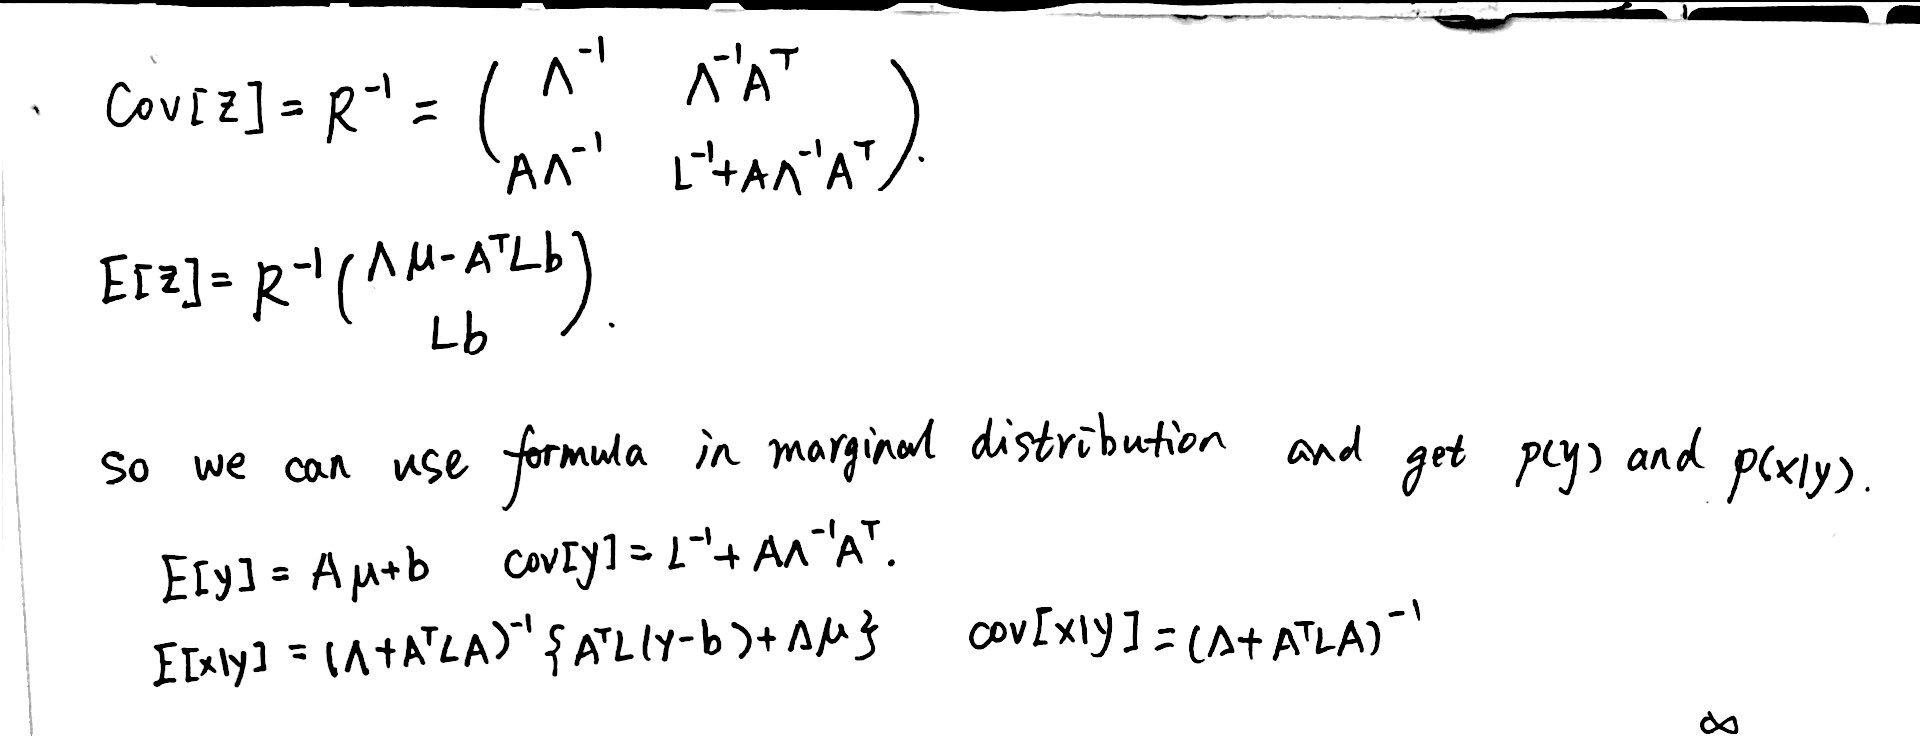
\includegraphics[width=\textwidth]{./imgs/GD1.jpg}
  \label{fig1.1}
\end{figure}
\subsection{Maximum likelihood for the Gaussian }
log likelihood function:
\begin{equation}\label{1.2.12}
  \ln p(\mathrm X|\mu,\Sigma) = -\frac{ND}2\ln(2\pi) - \frac N2\ln|\Sigma|-\frac12\sum_{n=1}^N(\mathrm x_n-\mu)^T\Sigma^{-1}(\mathrm x_n-\mu)
\end{equation}
we should pay attention that the thing on the exponent is a number and
\begin{equation}\label{1.2.13}
  (\mathrm x_n-\mu)^T\Sigma^{-1}(\mathrm x_n-\mu) = \mathrm x_n^T\Sigma^{-1}\mathrm x_n+\mu^T\Sigma^{-1}\mu-2\mathrm x_n^T\Sigma\mu
\end{equation}
\emph{sufficient statistics} for Gaussian distribution $\sum_{n=1}^N\mathrm x_n, \sum_{n=1}^N\mathrm x_n\mathrm x_n^T$ and  $\frac{\partial}{\partial \mu}\ln p(\mathrm X|\mu,\Sigma), \therefore\mu_{ML} = \frac1N\sum_{n=1}^N\mathrm x_n$\newline
$\Sigma_{ML}=\frac1N\sum_{n=1}^N(\mathrm x_n-\mu_{ML})(\mathrm x_n-\mu_{ML})^T $
\newline
and $\mathrm E[\mu_{ML}] =\mu, \mathrm E[\Sigma_{ML}] = \frac{N-1}{N}\Sigma$
\subsection{Sequential estimation}
$\mu_{ML}^{(N)}=\mu_{ML}^{(N-1)}+\frac1N(\mathrm x_N-\mu_{ML}^{(N-1)})$
we will not always be able to derive a sequential algorithm by this route, and so we seek a more general formulation of sequential learning, which  leads us to the \emph{Robbins-Monro} algorithm.
\begin{equation}\label{1.2.14}
  f(\theta) \equiv E[z|\theta] = \int zp(z|\theta)\mathrm dz
\end{equation}
\textbf{regression functions}
goal: to find root for $f(\theta) = 0$\newline
$$\theta^{(N)} = \theta^{(N-1)}+\alpha_{N-1}z(\theta^{(N-1)})$$
$z(\theta^{(N)})$ is an observe value of $z$ when $\theta$ takes the value $\theta^{(N)}$ and $\alpha_N$ should satisfy some conditions.\newline
\textbf{use Robbins Monro algorithm to solve maximizing log likelihood function problem}\newline
We want to get $$\frac{\partial}{\partial\theta}\{\frac{1}{N}\sum_{n=1}^N\ln p(\mathrm x_n|\theta)\} = 0$$
exchanging summation and derivative, taking the limit $N\rightarrow\infty$ and we have
$$\mathrm E_x[\frac{\partial}{\partial \theta}\ln p(x|\theta)]$$
so $$\theta^{(N)} = \theta^{(N-1)}+\alpha_{N-1}\frac{\partial}{\partial\theta^{(N-1)}}\ln p(x_N|\theta^{(N-1)})$$
\subsection{Baysesian inference for the Gaussian}
\begin{itemize}
  \item suppose $\sigma^2$ is known, to get $\mu$
  $$p(X|\mu) = \Pi_{n=1}^Np(x_n|\mu) = \frac1{(2\pi\sigma^2)^{N/2}}\exp\{-\frac1{2\sigma^2}\sum_{n=1}^N(x_n-\mu)^2\}$$
  we choose prior to be Gaussian, too
  $$p(\mu)= \mathcal N(\mu|\mu_0,\sigma_0^2) $$
so $$p(\mu|X) = \mathcal N(\mu|\mu_N,\sigma_N^2)$$
$$\mu_N  = \frac{\sigma^2}{N\sigma_0^2+\sigma^2}\mu_0+\frac{N\sigma_0^2}{N\sigma_0^2+\sigma^2}\mu_{ML}$$
$$\frac1{\sigma_N^2} = \frac1{\sigma_0^2}+\frac N{\sigma^2}$$
when N is infinite large, $\mu_N = \mu_{ML}$, only depend on observations, and $\sigma_N^2$ goes to 0 and the posterior distribution becomes infinitely peaked.\newline
if we take $\sigma_0^2$ to be infinite, so the prior is flat over all real numbers, so prior will be no use.\newline
sequential angle:
$$p(\mu|D)\propto [p(\mu)\Pi_{n=1}^{N-1}p(\mathrm x_n|\mu)]p(\mathrm x_N|\mu)$$
we can view the postrior distribution after N-1 observations as a prior distribution of the Nth observation.
  \item suppose $\mu$ is known, to get $\sigma^2$, see inference in figure\ref{fig1.2}
  \item suppose both are not known. see inference in figure\ref{fig1.3}
\end{itemize}
\begin{figure}
  \centering
  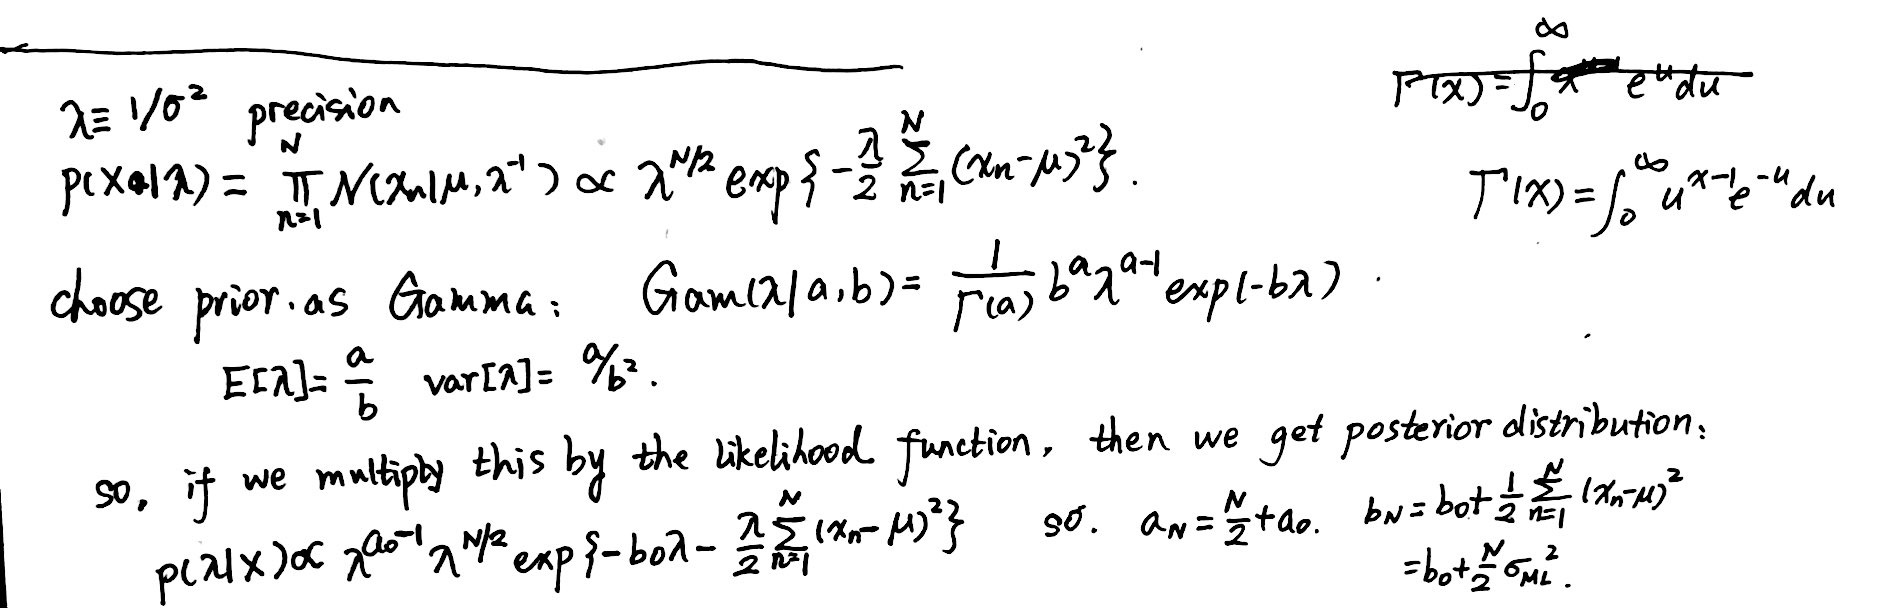
\includegraphics[width=\textwidth]{./imgs/GD2.jpg}
  \label{fig1.2}
\end{figure}
\begin{figure}
  \centering
  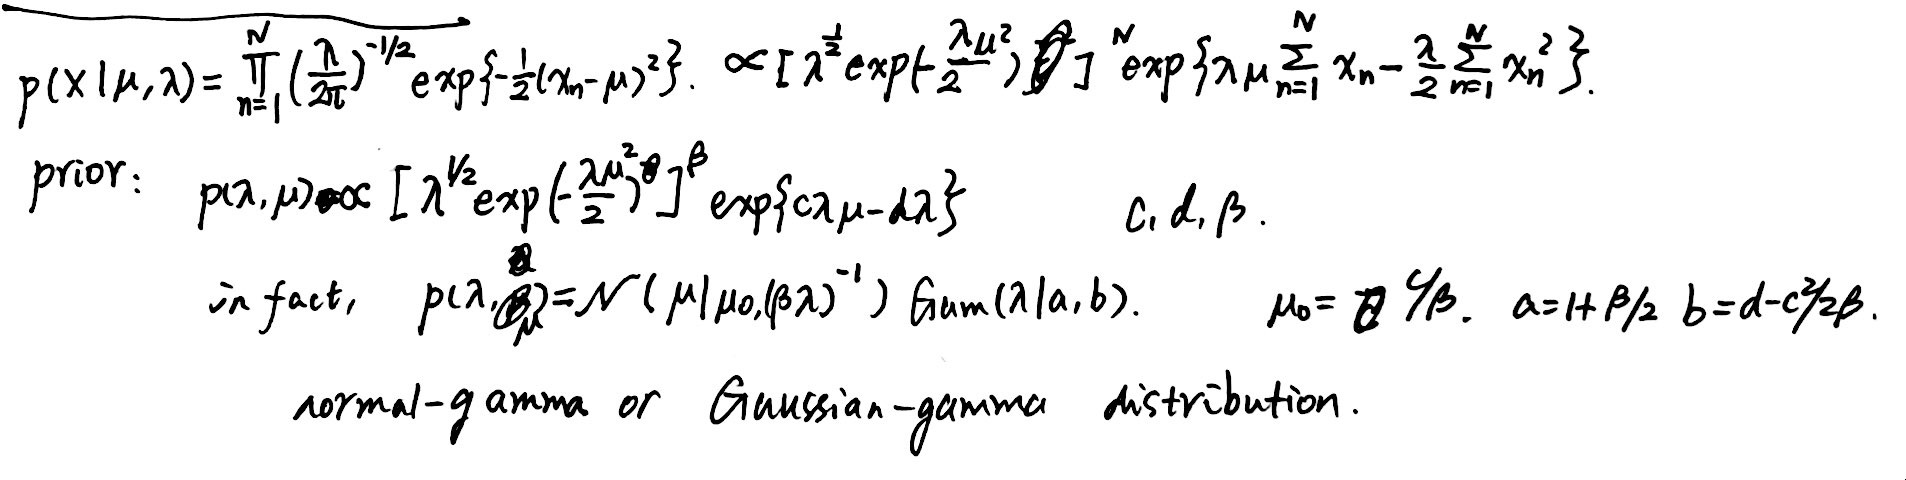
\includegraphics[width=\textwidth]{./imgs/GD3.jpg}
 \label{fig1.3}
\end{figure}
\subsection{Student's t-distribution}
precision $\lambda$    degrees of freedom $\nu$\newline
adding up an infinite number of Gaussian distribution having the same mean but different presicions, we can get Student's t-distribution.
$$\mathrm {St}[x|\mu,\lambda,\nu] = \frac{\Gamma(\nu/2+1/2)}{\Gamma(\nu/2)}{(\frac{\lambda}{\pi\nu})^{1/2}}[1+\frac{\lambda(x-\mu)^2}{\nu}]^{-\nu/2-1/2}$$
Data set: $(x_1,x_2,...,x_N)^T, (t_x,t_2,...,t_N)^T$.\newline
there is noise on the observation !
fit the data using a polynomial function:
\begin{equation}\label{2.1}
y(x, \textbf{w}) = w_0+w_1x+w_2x^2+\dots+w_Mx^M=\sum_{j=0}^Mw_jx^j
\end{equation}
this is a \textbf{linear} function of coefficients $\bf{w}$  !! so this is linear.
goal is to minimize:
\begin{equation}\label{2.2}
E(\textbf{w}) = \frac12\sum_{n=1}^N\{y(x_n,\textbf{w})-t_n\}^2
\end{equation}
\textit{this is a quadratic function of w so its derivatives with respect to coefficients will be linear so the minimization of the error function has a unique solution.}
\subsection{Mixtures of Gaussians}
$$p(\mathrm x) = \sum_{k=1}^K\pi_k\mathcal N(\mathrm x|\mu_k, \Sigma_k)$$
$$\sum_{k=1}^K \pi_k= 1$$

likelihood function:
$$\ln p(\mathrm X|\pi,\Sigma,\mu) = \sum_{n=1}^N\ln\{\sum_{k=1}^K\pi_k\mathcal N(\mathrm x_n|\mu_k,\Sigma_k)\}$$
this is more complex than a single Guassian because the presence of summation over $k$ inside the logarithm.  we can use EM algorithm later .

\section{The Exponential Family}
definition:
\begin{equation}\label{eq1.4.1}
  p(\mathrm x|\eta) = h(\mathrm x)g(\eta)\exp(\eta^T\mathrm u(\mathrm x))
\end{equation}
$g(\eta)$ is to normalize the function $g(\eta) \int h(\mathrm x)\exp(\eta^T\mathrm u(\mathrm x))\mathrm {dx} = 1$\newline
\textbf{Bernoulli}
\begin{equation}\label{1.4.2}
  p(x|\mu) =  \mu^x(1-\mu)^{1-x} = \exp\{x\ln\mu+(1-x)\ln(1-\mu)\} = (1-\mu)\exp\{\ln(\frac{\mu}{1-\mu})x\}
\end{equation}
so we define $\eta = \ln\frac{\mu}{1-\mu}$ so $\mu = \sigma(\eta) \frac{1}{1+\exp(-\eta)}$ \emph{logistic sigmoid function}
$u(x) = x, h(x) = 1, g(\eta) = \sigma(-\eta)$
\subsection{Maximum likelihood and sufficient statistics}
\begin{equation}\label{1.4.3}
  \mathrm  \nabla g(\eta) \int h(\mathrm  x)\exp\{\eta^T\mathrm  u(\mathrm  x)\}\mathrm  {dx} +g(\eta)\int h(\mathrm  x)\exp\{\eta^T\mathrm u(\mathrm x)\} \mathrm u(\mathrm  x) \mathrm {dx} = 0
\end{equation}
so $-\nabla \ln g(\eta) = \mathrm E[\mathrm  u(\mathrm  x)] $\newline
so consider
$$p(X|\eta)  = (\Pi_{n=1}^Nh(\mathrm  x_n))g(\eta)^N\exp\{\eta^T\sum_{n=1}^N\mathrm  u(\mathrm  x_n) \}$$
set the gradient to zero and we get
\begin{equation}\label{1.4.4}
  -\nabla \ln g(\eta_{ML} ) = \frac1N\sum_{n=1}^N\mathrm  u(\mathrm  x_n)
\end{equation}
$\sum_n\mathrm  u(\mathrm  x_n)$ is the sufficient statistics of the distribution.
\subsection{Conjugate priors}
for any member of the exponential family, there exist a conjugate  prior:
$$p(\eta|\chi, \nu) = f(\chi,\nu)g(\eta)^\nu\exp\{\nu\eta^T\chi\}$$
so the posterior distribution can be figured out as the same form:
$$p(\eta|X,\chi,\nu) \propto g(\eta)^{\nu+N}\exp\{\eta^T(\sum_{n=1}^N\mathrm  u(\mathrm  x_n)+\nu\chi)\}$$
\subsection{Noninformative priors}
to have little influence on the posterior distribution, we seek a form of prior distribution called \emph{a noninformative prior}.






\section{Laplace Approximation}\label{Laplace Appro}
In this chapter, we mainly want to solve the problem that when the posterior distribution is no longer Gaussian, how can we integrate exactly over the parameter vector $\ww $. So Laplace approximation can help us to transform a non-Gaussian distribution  into a Gaussian distribution. Consider first the case of a single continuous variable $z$, and suppose
\begin{equation}\label{}
  p(z) = \frac{1}{Z}f(z)
\end{equation}
where $Z = \int f(z)\md z$ is the normalization coefficient and is unknown. Our goal is to find a Gaussian approximation $q(z)$ which is centred on a mode of the distribution $p(z)$. To find a mode of $p(z)$, we set $p'(z)|_{z=z_0} = 0$, or equivalently
\begin{equation}\label{}
  \frac{\ud f(z)}{\ud z}|_{z=z_0}=0.
\end{equation}
Then due to the property of the log of Gaussian distribution, we consider a Taylor expansion of $\ln f(z)$ centred on the mode $z_0$ so that
\begin{equation}\label{}
  \ln f(z)\simeq \ln f(z_0) - \frac{1}{2}A(z-z_0)^2
\end{equation}
where
\begin{equation}\label{}
  A = -\frac{\ud^2}{\ud z^2}\ln f(z)|_{z=z_0}.
\end{equation}
Then
\begin{equation}\label{}
  f(z) \simeq \hat f(z) = f(z_0)\exp\{-\frac A2(z-z_0)^2\}.
\end{equation}
Making normalization over $\hat f(z)$, we have
\begin{equation}\label{}
  q(z) = \frac{A}{2\pi}^{1/2}\exp\{-\frac A2(z-z_0)^2\}.
\end{equation}
Note that the Gaussian approximation is only be well defined when $A>0$, in other words, the stationary point $z_0$ must be a local maximum.

Then we want to extend to $M$-dimensional space $\zz$ and $p(\zz) = \frac 1Zf(\zz)$. At a stationary $\zz_0$ the gradient $\nabla f(\zz) =0$. Similarly
\begin{equation}\label{}
  \ln f(\zz) \simeq \ln f(\zz_0)-\frac12(\zz-\zz_0)\trans \mbf A(\zz-\zz_0)
\end{equation}
where the $M\times M$ Hessian matrix $\mbf A$ is defined by
\begin{equation}\label{}
  \mbf A = -\nabla\nabla\ln f(\zz)|_{\zz=\zz_0}.
\end{equation}
Taking the exponential of the both side, we obtain
\begin{equation}\label{}
  f(\zz) \simeq f(\zz_0)\exp\{-\frac12(\zz-\zz_0)\trans\mbf A(\zz-\zz_0)\}.
\end{equation}
Making normalization, we have
\begin{equation}\label{}
  q(\zz) = \frac{|\mbf A|^{1/2}}{(2\pi)^{M/2}}\exp\{-\frac12(\zz-\zz_0)\trans\mbf A(\zz-\zz_0)\} = \normD(\zz|\zz_0,\mbf A^{-1}).
\end{equation}
This Gaussian distribution is only well defined when its \textit{precision matrix}, given by $\mbf A$, is positive definite.

Note that the normalization constant $Z$ of the true distribution does not need to be known in order to apply the Laplace method. As a result of the central limit theorem, the posterior distribution for a model is expected to become increasingly better when the number of data points is increased, so we would expect the Laplace approximation to be most useful when the number of data points is relatively large.
\subsubsection*{Model comparison and BIC}
This section illustrates \textit{Occam factor} and \textit{BIC} in view of the Laplace approximation, more details can be found in section 4.4.1 of \textit{PRML}.


\section{Jacobian Matrix and Hessian Matrix}\label{Matrix}
\section{FOR NEW}

\chapter{Models}
\section{Polynomial Curve Fitting}
$\textbf{x} = (x_1,x_2,\dots, x_N)^T $ and $\textbf{t} =(t_1,t_2, \dots, t_N)^T$
There is noise on the observation !\newline
Fit the data using a polynomial function:
$$y(x, \textbf{w}) = w_0+w_1x+w_2x^2+\dots+w_Mx^M=\sum_{j=0}^Mw_jx^j$$
This is a \textbf{linear} function of coefficients \textbf{w}  !! So this is linear.\newline
Goal is to minimize:
$$E(\textbf{w}) = \frac12\sum_{n=1}^N\{y(x_n,\textbf{w})-t_n\}^2$$
This is a quadratic function of $\ww$ so its derivatives with respect to coefficients will be linear so the minimization of the error function has a unique solution.
\subsection{the influence of order M}
define error by root-mean-square:
\begin{equation}\label{2.3}
E_{RMS} = \sqrt{2E(\textbf{w}^*)/N}:
\end{equation}
too small: not enough.\newline
too large: \textbf{overfitting} and large coefficients, very sensitive to \textbf{noise}! low training error while large testing error.
\subsection{the influence of size of training set}
increasing the size of the data set reduces the over-fitting priblem.\newline
\textit{comment}: this is obvious because the when the size of data set gets larger, the order will become smaller relatively. the requirement for over-fitting is larger order. but when we choose the complexity of our model, we can not depend on the size of data set, we must choose more robust model for \textbf{specific problem}.
\subsection{modifying error function to solve overfitting}
\begin{equation}\label{2.4}
\tilde{E}(\textbf{w}) = \frac12\sum_{n=1}^M\{y(x_n,\textbf{w})-t_n\}^2+\frac{\lambda}{2}||\textbf{w}||^2
\end{equation}
\textit{regularizier} $$||\textbf{w}||^2 = w_0^2+\dots+w_M^2$$
\textit
{somtimes $w_0$ is omitted to exclude the effect of origin for the tarfet variable !!}
in nerual networks, this approach is known as \textit{weight decay}
To optimize $M$ and $\lambda$, we sometimes divide dataset into \textit{training} and \textit{validation} but this is a waste, so we need more sophisticated approaches.

\section{Linear Models for Regression}
\subsection{Linear Basis Function Models}
input $\mathrm x\in R^D$
\begin{equation}\label{eq2.2.1}
  y(\mathrm x,\mathrm w) = w_0+w_1x_1+\dots +w_Dx_D
\end{equation}
extend to nonlinear function of $\mathrm x$ and $y(\mathrm x,\mathrm w) =\mathrm w^T\phi(\mathrm x)$, there are M basis functions $\phi_j(\mathrm x), j=1,2\dots,M$ and $\phi_0(\mathrm x) = 1$\newline
so $\mathrm w\in R^M$
\textbf{normal basis functions}
\begin{itemize}
  \item polynomial $\phi_j(x) = x$
  \item Gaussian $\phi_j(x) = \exp\{-\frac{(x-\mu_j)^2}{2s^2}\}$
  \item sigmoidal $\phi_j(x) = \sigma(\frac{x-\mu_j}{s}) , \sigma(a) = \frac1{1+\exp(-a)}$ sigmoid is equivalent to 'tanh' function.
\end{itemize}
\subsubsection{Maximum likelihood and least squares}
$$t = y(\mathrm x,\mathrm w)+\epsilon, \epsilon\sim\mathcal N(0,\beta^{-1}), \beta = \sigma^{-2}$$
so $$p(t|\mathrm x,\mathrm w,\beta) = \mathcal N(t|y(\mathrm x,\mathrm w),\beta^{-1})=\frac{1}{\sqrt{2\pi/\beta}}\exp\{-\frac{\beta(t-y(\mathrm x,\mathrm w))^2}{2}\}$$
$$\mathrm E[t|\mathrm x] =\int t p(t|\mathrm x)\mathrm dt=y(\mathrm x,\mathrm w)$$
for $N$ observations,
$$p(\mathrm t|\mathrm X,\mathrm w,\beta) = \Pi_{n=1}^N\mathcal N(t_n|\mathrm w^T\phi(\mathrm x_n), \beta^{-1})$$
we can ignore $\mathrm X$ in he condition and get likelihood function:
$$\ln p(\mathrm t|\mathrm w,\beta) = \sum_{n=1}^N\ln \mathcal N(t_n|\mathrm w^T\phi(\mathrm x_n),\beta^{-1}) = \frac N2\ln\beta-\frac N2\ln(2\pi)-\beta E_D(\mathrm w)$$
in which, $$E_D(\mathrm w) = \frac12\sum_{n=1}^N\{t_n-\mathrm w^T\phi(\mathrm x_n)\}^2$$
use maximum likelihood to determine $\mathrm w$ and $\beta$, we get
\begin{equation}\label{3.2.2}
  \nabla \ln p(\mathrm t|\mathrm w,\beta) = \sum_{n=1}^N\{t_n-\mathrm w^T\phi(\mathrm x_n)\}\phi(\mathrm x_n)^T = 0
\end{equation}
and we obtain
\begin{equation}\label{}
  \mathrm w_{ML} = (\Phi^T\Phi)^{-1}\Phi^T\mathrm t
\end{equation}
here $\Phi$ is an $N\times M$ matrix called the \textit{design matrix}, and $\Phi_{nj} = \phi_j(\mathrm x_n)$
so each row of $\Phi$ is dependent on the same observation and each column is dependent on the same basis function. \newline
$\Phi^{\dagger} = (\Phi^T\Phi)^{-1}\Phi^T$ is known as the \textit{Moore-Penrose pseudo-inverse} of the matrix.\newline
For $w_0$, we can see $w_0=\bar t-\sum_{j=1}^{M-1}w_j\bar \phi_j$, where $\bar t=\frac1N\sum_{n=1}^Nt_n, \bar{\phi_j}=\frac1N\sum_{n=1}^N\phi_j(\mathrm x_n)$. So the bias $w_0$ compensates for the different between the averages of the target values and the weighted sum of the averages of the basis function values. Also we can get$1/\beta_{ML}=\frac1N\sum_{n=1}^N\{t_n-\mathrm w_{ML}^T\phi(\mathrm x_n)\}^2$
\subsubsection{Geometry of least squares}
$\mathrm t=(t_1,\dots,t_N)^T$ is a vector in N-dimensional space. Define $\mathrm y$ to be an N-dimensional vector whose $n^{th}$ element is given by $y(\mathrm x_n,\mathrm w)$,  so $\mathrm y$ is an arbitrary linear combination of the vectors $\varphi_j$, it can live anywhere in the M-dimensional subspace.\newline
Thus the least-squares solution for $\mathrm  w $ corresponds to that choice of $\mathrm y$ that lies in subspace $S$ and that is closest to t. so we choose the orthogonal projection of $\mathrm t$  onto the subspace.\newline
some problems: singularity of $\Phi^T\Phi$
\subsubsection{Sequential learning}
SGD (\textit{stochastic gradient descent}, aka, \textit{sequential gradient descent})\newline
$$\mathrm w^{(\tau+1)}=\mathrm w^{(\tau)}-\eta\nabla E_n$$
So for the case of the sum-of-squares erroe function, this gives
$$\mathrm w^{\tau+1}=\mathrm w^{(\tau)}+\eta(t_n-\mathrm w^{(\tau)^T}\phi_n)\phi_n$$ where $\phi_n=\phi(\mathrm x_n)=(\phi_1(\mathrm x_n), \dots, \phi_M(\mathrm x_n))^T$
\textit{least-mean-squares} algorithm (\textit{LMS})
\subsubsection{Regularized least squares}
Total error function to be minimized takes the from :
$E_D(\mathrm w) +\lambda E_W(\mathrm w)$ Usually, $E_W(\mathrm w) = \frac12\mathrm w^T\mathrm w$ And we can obtain $\mathrm w=(\lambda\mathrm I+\Phi^T\Phi)^{-1}\Phi^T\mathrm t$ by setting the gradient of total error function with respect to $\mathrm w$ to zero.
\subsubsection{Multiple outputs}
$\mathrm t\in R^K, K>1$ is the outputs.\newline
$\mathrm y(\mathrm x,\mathrm W) =W^T\phi(\mathrm x)$
$W\in R^{M\times K }, \phi(\mathrm x)$ is a $M$-dimensional column vector with elements $\phi_j(\mathrm x)$ with $\phi_0(\mathrm x) = 1$.\newline
$M$: the number of basis functions $\phi_1(\mathrm x), \dots, \phi_M(\mathrm x)$\newline
$K$: outputs are in K-dimensional space.
$$p(\mathrm t|\mathrm x,\mathrm W,\beta) = \mathcal N(\mathrm t|\mathrm W^T\phi(\mathrm x),\beta^{-1}\mathrm I)$$
If we have $N$ observations, $\mathrm t_1,\dots,\mathrm t_N$, into one matrix $\mathrm T\in R^{N\times K}$, combine $\mathrm x_1,\dots,\mathrm x_N$  into one  matrix $\mathrm X\in R^{N\times D}$
\begin{equation}\label{eq2.2.3}
  \ln p(\mathrm T|\mathrm X,\mathrm W,\beta) = \sum_{n=1}^N\ln\mathcal N(\mathrm t_n|\mathrm W^T\phi(\mathrm x_n), \beta^{-1}\mathrm I) = \frac{NK}{2}\ln(\frac{\beta}{2\pi})-\frac{\beta}{2}\sum_{n=1}^N||\mathrm t_n-\mathrm W^T\phi(\mathrm x_n)||^2
\end{equation}
and we can get $\mathrm W_{ML} = (\Phi^T\Phi)^{-1}\Phi^T\mathrm T$, $\mathrm w_k = (\Phi^T\Phi)^{-1}\Phi^T\mathrm t_k$

\subsection{The Bias-Variance Decomposition}
Recall Section1.5.5 in PRML, which gave us the expected loss in regression problem:
\begin{equation}\label{}
\mathbb{E}[L]=\iint L(t,y(\xx))p(\xx,t)\mrm d\xx\mrm dt
\end{equation}
To minimize $\mathbb E[L]$ we set
\begin{equation}\label{}
  y(\xx) = \mathbb E_t[t|\xx]
\end{equation}
then we can rewrite the loss function:
\begin{gather}\label{}
L =  \{y(\xx)-t\}^2 = \{y(\xx) - \mathbb E[t|\xx] + \mathbb E[t|\xx] -t\}^2 \\
  =\{y(\xx)-\Exp[t|\xx]\}^2+2\{y(\xx)-\Exp[t|\xx]\}\{\Exp[t|\xx]-t\}+\{\Exp[t|\xx]-t\}^2
\end{gather}
Then, the expected loss is:
\begin{equation}\label{}
\Exp[L] = \int\{y(\xx)-\Exp[t|\xx]\}^2p(\xx)\mrm d\xx+\iint \{\Exp[t|\xx]-t\}^2p(\xx)\mrm d\xx\mrm dt.
\end{equation}
Denote $h(\xx) = \Exp[t|\xx]$, the second term is independent of $y(\xx)$, and arises from the intrinsic noise on the data. So we can only minimize the first term. And this term is nonnegative and if we get $h(\xx)$, we can set $y(\xx) = h(\xx)$ and we'll get a minimal loss. But because of limited training data points and limited computational sources, we can never get exact $h(\xx)$, and we want to learn an optimal $y(\xx)$ from the training data.

Now suppose we have a number of data sets of the same size $N$ and each drawn independently from the true distribution $p(\xx,t)$. For each data set, we can get a regression function $y(\xx;\mathcal D)$, and for each particular data set, the first term takes the form as:
\begin{equation}\label{}
  \{y(\xx;\calD)-h(\xx)\}^2
\end{equation}
And we denote the expectation of the function value over all the data sets as $ \Exp_{\calD}[y(\xx;\cal D)]$, then
\begin{gather}\label{}
  \{y(\xx;\calD)-h(\xx)\}^2 = \{y(\xx;\calD)-\Exp_{\calD}[y(\xx;\calD]+\Exp_{\calD}[y(\xx;\calD]-h(\xx)\}^2 \\
\end{gather}
So,
\begin{gather}\label{}
  \Exp_\calD[\{y(\xx;\calD)-h(\xx)\}^2] \\
  = \{\Exp_\calD[y(\xx;\calD)-h(\xx)\}^2 +\Exp_\calD[\{y(\xx;\calD)-\Exp_\calD[y(\xx;\calD]\}^2]
\end{gather}
The first term, called squared \textit{bias} represents the extent to which the average prediction over all data sets differ from the desired regression function. The second term, called the \textit{variance}, measures the extent to which the solutions for individual data sets vary around their average, and hence it measures the extent to which the function $y(\xx;\calD$ is sensitive to the choice of data set.

To sum up, the expected squared loss is:
\begin{equation}\label{}
  \mrm{expected loss} = (\mrm{bias})^2+\mrm{variance}+\mrm{noise}.
\end{equation}
There is a trade-off between bias and variance.  If a model is very flexible, it will lead to very low bias while high variance, and if a model is very rigid, it will lead to very low variance while high bias.

\textit{There is an example in PRML section3.2 illustrating the trade-off between bias and variance.}

\subsection{Bayesian Linear Regression}
Because effective model complexity, governed by the number of basis functions, needs to be controlled according to the size of the data set, the issue of deciding the appropriate model complexity for the particular problem which cannot be decided simply maximizing the likelihood function still exists. So we turn to Bayesian treatment of linear regression and we can avoid the over-fitting problem and also lead to automatic methods of determining model complexity using the training data alone.
\subsubsection{Parameter distribution}
we assume that precision parameter $\beta$ is known and the prior  probability distribution is as the form:
\begin{equation}\label{eq2.2.4}
  p(\mathrm w) =\mathcal N(\mathrm w|\mathrm m_0,\mathrm S_0)
\end{equation}
so the posterior probability will be Gaussian, too
\begin{equation}\label{eq2.2.5}
  p(\mathrm w|\mathrm t) = \mathcal N(\mathrm w|\mathrm m_N,\mathrm S_N)
\end{equation}
where $\mathrm m_N=\mathrm S_N(\mathrm S_0^{-1}\mathrm m_0+\beta \Phi^T\mathrm t)$ and $\mathrm S_N^{-1}=\mathrm S_0^{-1}+\beta\Phi^T\Phi$\newline
To simplify the model we assume $\mathrm S_0 = \alpha^{-1}\mathrm I$ and $ \mathrm m_0=\mathrm 0$. Then, maximization of this posterior distribution with respect to $\mathrm w$ is therefore equivalent to minimization of the sum-of-square error function with the addition of a quadratic regularization term.
\subsubsection{Predictive distribution }
In practice, we only want to predict t for new values of $\mathrm x$ rather than $\mathrm w$. So we evaluate the \textit{predictive distribution} defined by
\begin{equation}\label{eq2.2.6}
  p(t|\mathrm t,\alpha,\beta) = \int p(t|\mathrm w,\beta)p(\mathrm w|\mathrm t,\alpha,\beta)\mathrm {dw}
\end{equation}
\subsubsection{Equivalent kernel }
We see that the predictive mean can be written in the form
$$y(\mathrm x,\mathrm m_N) =\mathrm m_N^T\phi(\mathrm x)=\beta\phi(\mathrm x)^T\mathrm S_N\Phi^T\mathrm t=\sum_{n=1}^N\beta\phi(\mathrm x)^T\mathrm S_N\phi(\mathrm x_n)t_n$$
we can define kernel
$k(\mathrm x,\mathrm x') = \beta\phi(\mathrm x)^T\mathrm S_N\phi(\mathrm x')$ is known as the *smoother matrix* or *equivalent kernel*. make predictions by taking linear combinations of the training set target values.
\subsection{Bayesian Model Comparison}
Consider the problem of model selection from a Bayesian perspective by simply involving the use of probabilities to represent uncertainty in the choice of model.\newline
Given a training seet $\mathcal D$ we wish to evaluate the posterior distribution $p(\mathcal M_i|\mathcal D) \propto p(\mathcal M_i)p(\mathcal D|\mathcal M_i)$\newline
the prior shows our preference for different models.\newline
If we choose $p(\mathcal M_i)$ to be identical, then the interesting term is the model evidence $p(\mathcal D|\mathcal M_i)$.\newline
the model evidence is sometimes called \textit{marginal likelihood.}
We can conclude that the Bayesian framework avoids the problem of over-fitting  and allows models to be compared on the basis of the training data alone. However, we still needs to make assumptions about the form of the model.
\subsection{The Evidence Approximation}
If we introduce hyperpriors over $\alpha$ and $\beta$, the predictive distribution is obtained by marginalizing over $\ww$, $\alpha$ and $\beta$:
\begin{equation}\label{}
  p(t|\ttt)=\iiint p(t|\ww,\beta)p(\ww|\ttt,\beta)p(\alpha,\beta|\ttt)\mrm d\ww\mrm d\alpha\mrm d\beta.
\end{equation}
We omitted the input variable $\xx$ to keep the notation uncluttered. This integration can not be analytically computed so we use approximation in which we set the hyperparameters to specific values determined by maximizing the marginal likelihood function obtained by first integrating over $\ww$. This frame work is known in the statistics literature as \textit{empirical Bayes} or \textit{type 2 maximum likelihood} or \textit{generalized maximum likelihood}, and in machine learning literature is also called \textit{evidence approximation}.

The marginal likelihood function $p(\ttt|\alpha,\beta)$ is obtained by integrating over weight parameters $\ww$, so that
\begin{equation}\label{}
  p(\ttt,\alpha,\beta) = \int p(\ttt|\ww,\beta)p(\ww|\alpha)\mrm d\ww.
\end{equation}
Using conditional distribution in linear-Gaussian model, we finally can write the log of marginal likelohood in the form
\begin{equation}\label{eq2.2.8}
  \ln p(\ttt|\alpha, \beta) = \frac M2\ln \alpha +\frac N2\ln\beta-E(\mbf m_N)-\frac12\ln|\mbf A|-\frac N2\ln(2\pi)
\end{equation}
in which
\begin{gather}\label{eq2.2.7}
  E(\mbf m_N) = \frac{\beta}{2}\|\ttt-\Phi\mbf m_N\|^2+\frac\alpha2\mbf m_N^\mrm T\mbf m_N \\
  \mbf A=\nabla\nabla E(\ww) \\
  \mbf m_N=\beta \mbf A\rev \Phi \trans\ttt.
\end{gather}
\subsubsection*{Maximizing the evidence function}
First consider maximization of $p(\ttt|\alpha, \beta)$ w.r.t $\alpha$. From eq.\ref{eq2.2.7}, assume
\begin{equation}\label{}
  (\beta\Phi\trans\Phi)\uu_i=\lambda_i\uu_i
\end{equation}
then $\mbf A$ has eigenvalues $\alpha +\lambda_i$.
\begin{equation}\label{}
  \frac{\ud}{\ud \alpha}\ln|\mbf A|=\frac{\ud}{\ud\alpha}\ln\prod_{i}(\lambda_i+\alpha)=\frac{\ud}{\ud\alpha}\sum_i\ln(\lambda_i+\alpha)=\sum_i\frac1{\lambda_i+\alpha}
\end{equation}
So the stationary points of eq.\ref{eq2.2.8} w.r.t. $\alpha$ satisfy:
\begin{equation}\label{}
  0=\frac{M}{2\alpha}-\frac12\mm_N\trans\mm_N-\frac12\sum_i\frac1{\lambda_i+\alpha}.
\end{equation}
So
\begin{gather}\label{}
  \alpha\mm_N\trans\mm_N=M-\alpha\sum_i\frac1{\lambda_i+\alpha}=\gamma.\\
  \gamma = \sum_{i}\frac{\lambda_i}{\alpha+\lambda_i}
\end{gather}
and
\begin{equation}\label{}
  \alpha = \frac{\gamma}{\mm_N\trans\mm}
\end{equation}
Note that this is an implicit solution for $\alpha$ since $\gamma$ and $\mm_N$ are both dependent of $\alpha$.  And we can compute $
alpha$ by lots of iterations until convergence of $\alpha$, $\gamma$ and $\mm_N$.

Then we can similarly maximize the log likelihood function w.r.t $\beta$. Notice that the eigenvalues $\lambda_i$ is defined proportional to $\beta$, and hence $\ud\lambda_i/\ud\beta=\lambda_i/\beta$, so
\begin{equation}\label{}
  \frac{\ud}{\ud \beta}\ln|\mbf A|=\frac{\ud}{\ud\beta}\sum_i\ln(\lambda_i+\alpha)=\frac{1}{\beta}\sum_i\frac{\lambda_i}{\lambda_i+\alpha}=\frac{\gamma}{\beta}
\end{equation}
finally
\begin{equation}\label{}
    \frac{1}{\beta} = \frac{1}{N-\gamma}\sum_{n=1}^{N}\{t_n-\mm_N\trans\phi(\xx_n)\}^2.
\end{equation}
This is also an implicit solution for $\beta$.

\subsection{Limitations of Fixed Basis Functions}
basis function $\phi_j(\mathrm x)$ are fixed before the training data set is observed.\newline
curse of dimensionality




\section{Linear Models for Classification}
This chapter aims to solve classification tasks linear models.\newline
Three approaches:
\begin{itemize}
  \item discriminant function, directly assigns each vector $\mathrm x$ to a specific class.
  \item models conditional probability distribution $p(\mathcal C_k|\mathrm x)$ in an inference stage and then subsequently uses this distribution to make optimal decisions:
      \begin{itemize}
        \item directly model the conditional probability
        \item generative approach. model the class-conditional densities given by $p(\mathrm x|\mathcal C_k)$, together with the prior probabilities $p(\mathcal C_k)$
      \end{itemize}
\end{itemize}

For classification problem, we consider to generalize a linear model by transform the linear function of $\ww$ using a nonlinear  function $f(\cdot)$ so that
\begin{equation}\label{}
  y(\xx) = f(\ww\trans\xx+w_0)
\end{equation}
In the machine learning literature $f(\cdot)$ is known as \textit{activation function}, whereas its inverse is called a \textit{link function} in statistics literature. So the model is no longer linear in the parameters due to the presence of the nonlinear activation function.
\subsection{Discriminant Functions}
\begin{equation}\label{}
y(\xx) = \ww^T\xx+w_0
\end{equation}
For two-class situation,  the normal distance from the origin to the decision surface is given by is given by
\begin{equation}\label{}
  \frac{ \ww^T\xx}{||\ww||} = -\frac{w_0}{||\ww||}
\end{equation}
for multiple classes,  it's kind of difficult to reduce to 2-class. a single $K$-class discriminant comprising $K$ linear functions of the form:
$y_k(\mathrm x) = \mathrm w_k^T\mathrm x+w_{k0}$ and then assigning a point $\mathrm x$ to class $\mathcal C_k$ if $y_k(\mathrm x)$ is the largest.\newline
approaches to learning the discriminant functions:
\begin{itemize}
  \item least squares for classification
  \item fisher's linear discriminant
  \item perceptron algorithm
\end{itemize}
\subsubsection*{Least squares for classification}
We have $K$ classes and each class $\cal C_k$ is described by its own linear model so that
\begin{equation}\label{}
  y_k(\xx)=\ww_k\trans\xx+w_{k0}.
\end{equation}
Using vector notation we can rewrite it in the form of:
\begin{equation}\label{}
  \yy(\xx)=\tilde{\WW}\trans\tilde{\xx}
\end{equation}
where $\tilde{\WW}$ is a matrix whose $k^{\mrm{th}}$ column comprises the $D+1$-dimensional vector $\tilde{\ww}_k=(w_{k0}, \ww_k\trans)\trans$ and $\tilde{\xx}$ is the corresponding augmented input vector $(1,\xx\trans)\trans$. A new input $\xx$ is then assigned to the class for which the output $y_k=\tilde{\ww}\trans\tilde{\xx}$ is the largest.

We now determine $\tilde{\WW}$  by minimizing a sum-of-square error function:
\begin{equation}\label{}
  E_D(\tilde{\WW})=\frac12\mrm{Tr}\{(\tilde{\XX}\tilde{\WW}-\TT)\trans(\tilde{\XX}\tilde{\WW}-\TT)\}
\end{equation}
where $\TT$ is defined as a matrix whose $n^{\mrm{th}}$ row is the vector $\ttt_n\trans$ and $\tilde{\XX}$ is a matrix whose $n^{\mrm{th}}$ row is $\tilde{\xx}_n\trans$. We then obtain the solution for optimal $\tilde{\WW}$ in the form
\begin{equation}\label{}
  \tilde{\WW}=(\tilde{\XX}\trans\tilde{\XX})\rev\tilde{\XX}\trans\TT=\tilde{\XX}^\dagger\TT
\end{equation}

Least square model fails obviously because when we recall that it correspond to maximum likelihood under the assumption of a Gaussian conditional distribution, whereas binary target vectors clearly have a distribution that is far from Gaussian.
\subsubsection*{Fisher's linear discriminant}
Here we consider classification problem in the view of dimension reduction.

Consider two-class problem first, we can select a projection that maximizes the class separation. Assume there are $N_1$ points in class $\mcal C_1$ and $N_2$ points in class $\mcal C_2$, define mean vectors:
\begin{equation}\label{}
  \mm_1=\frac1{N_1}\sum_{n\in\mcal C_1}\xx_n, \ \ \mm_2 = \frac{1}{N_2}\sum_{n\in\mcal C_2}\xx_n.
\end{equation}
So projection class means will be:
\begin{equation}\label{}
  m_k=\ww\trans\mm_k,\ k=1,2
\end{equation}
and we want to maximize
\begin{equation}\label{}
  m_2-m_1=\ww\trans(\mm_2-\mm_1).
\end{equation}
This can be arbitrarily large simply by increasing the magnitude of $\ww$. So we add a constraint $\sum_iw_i^2=1$, and then using Lagrange multiplier we obtain $\ww\propto(\mm_2-\mm_1)$. But this approach is not robust because some well separated samples in original two-dimensional space could overlapping after projected onto the vector $\mm_2-\mm_1$. So Fisher's linear discriminant want to solve this problem.

The idea proposed by Fisher is to maximize a function that will give a large separation between the projected class means while also giving a small variance within each class, thereby minimize the class overlap. We define
\begin{equation}\label{}
  s_k^2=\sum_{n\in\mcal C_k}(y_n-m_k)^2
\end{equation}
which is the within class $\mcal C_k$ variance, where $y_n=\ww\trans\xx_n$. And \textit{Fisher criterion} is defined by
\begin{equation}\label{}
  J(\ww) = \frac{(m_2-m_1)^2}{s_1^2+s_2^2} = \frac{\ww\trans\mbf S_\mB\ww}{\ww\trans\mbf S_\mW\ww}
\end{equation}
where $\mbf S_\mB$ is the \textit{between-class} covariance matrix
\begin{equation}\label{}
  \mbf S_\mB = (\mm_2-\mm_1)(\mm_2-\mm_1)\trans
\end{equation}
and $\mbf S_\mW$ is the \textit{within-class} covariance matrix
\begin{equation}\label{}
  \mbf S_\mW = \sum_{n\in\mcal C_1}(\xx_n-\mm_1)(\xx_n-\mm_1)\trans+\sum_{n\in\mcal C_2}(\xx_n-\mm_2)(\xx_n-\mm_2)\trans.
\end{equation}
We find that $J$ is maximized when
\begin{equation}\label{}
  (\ww\trans\mbf S_\mB\ww)\mbf S_\mW\ww=(\ww\trans\mbf S_\mW\ww)\mbf S_\mB\ww.
\end{equation}
Since do not care about the magnitude of $\ww$, we obtain
\begin{equation}\label{}
  \ww\propto\mbf S_\mW\rev(\mm_2-\mm_1).
\end{equation}

Now we consider the relation between Fisher's discriminant and least squares. If we adopt a slightly different (in contrast to 1-of-K coding)target encoding scheme, then the least-squares solution for the weights becomes equivalent to the Fisher solution. More details can be found in section4.1.5 of \textit{PRML}.

As for K-classes situation, the solution is similar to 2-classes situation and more details can be found in section4.1.6 of \textit{PRML}.


\subsubsection*{The perceptron algorithm}
We choose the nonlinear activation function $f(\cdot)$ to be a step function of the form
\begin{equation}\label{}
  f(a) = \left\{
  \begin{array}{c}
    +1,\ a\geq 0 \\
    -1,\  a<0.
  \end{array}
  \right .
\end{equation}

The algorithm used to determine the parameters $\ww$ of the perceptron can most easily be motivated by error function minimization. A natural choice for error function is the total number of misclassified patterns. However this error function is discontinuous at some points while the gradient is zero all everywhere.

We therefore consider an alternative error function as \textit{perceptron criterion}. For right predicted input, we have
\begin{equation}\label{}
  \ww\trans\phi(\xx_n)t_n > 0.
\end{equation}
The perceptron criterion is therefore given by
\begin{equation}\label{}
  E_p(\ww)=-\sum_{n\in mcal M}\ww\trans\phi_nt_n
\end{equation}
where $\mcal M$ denotes the set of all misclassified patterns. Then the change in the weight vector $\ww$ is given by
\begin{equation}\label{}
  \ww^{(\tau+1)}=\ww^{(\tau)} - \eta\nabla E_p(\ww)=\ww^{(\tau)}+\eta\phi_nt_n.
\end{equation}

\subsection{Probabilistic Generative Models}
Here we shall adopt a generative approach in which we model the class-conditional densities $p(\xx|\mcal C_k)$, as well as the class prior $p(\mcal C_k$, and then we want to compute posterior $p(\mcal C_k|\xx)$.

Consider 2-classes case first, we have
\begin{equation}\label{}
  p(\mcal C_1|\xx) = \frac{p(\xx|\mcal C_1)p(\mcal C_1)}{p(\xx|\mcal C_1)p(\mcal C_1)+p(\xx|\mcal C_2)p(\mcal C_2)}.
\end{equation}
Then we define
\begin{equation}\label{}
  a = \ln\frac{p(\xx|\mcal C_1)p(\mcal C_1)}{(\xx|\mcal C_2)p(\mcal C_2)}
\end{equation}
so
\begin{equation}\label{eq2.3.1}
  p(\mcal C_1|\xx) = \frac{1}{1+\exp(-a)}=\sigma(a).
\end{equation}
And we call $\sigma(a) = \frac{1}{1+\exp(a)}$ \textit{logistic sigmoid} function. The inverse of the sigmoid function is given by
\begin{equation}\label{}
  a = \ln(\frac{\sigma}{1-\sigma})
\end{equation}
and is known as the \textit{logit} function. It represents the log of the ratio of probabilities $\ln [p(\mcal C_1|\xx)/p(\mcal C_2|\xx)]$ for the two classes, also known as the \textit{log odds}.

Given eq.\ref{eq2.3.1}, we shall shortly consider situations in which $a(\xx)$ is a linear function of $\xx$, in which case the posterior probability is governed by a generalized linear model.

For $K>2$ classes, we have
\begin{equation}\label{}
  p(\mcal C_k|\xx)=\frac{p(\xx|\mcal C_k)p(\mcal C_k)}{\sum_jp(\xx|\mcal C_j)p(\mcal C_j}=\frac{\exp(a_k)}{\sum_j\exp(a_j)}
\end{equation}
where $a_k$ is defined by
\begin{equation}\label{eq2.3.2}
  a_k = \ln p(\xx|\mcal C_k)p(\mcal C_k).
\end{equation}
The normalized exponential is also known as the \textit{softmax function}.

Then, we'll investigate the consequences of choosing specific forms for the class-conditional densities, looking first at continuous input variables $\xx$ and then discussing briefly the case of discrete inputs.

For continuous input, let us assume that the class-conditional densities are Gaussian and firstly assume that all classes share the same covariance matrix.
\begin{equation}\label{}
  p(\xx|\cat_k)=\frac{1}{(2\pi)^{D/2})}\frac1{|\Sigma|^{1/2}}\exp\{-\frac12(\xx-\bmu_k)\trans\Sigma\rev(\xx-\bmu_k)\}
\end{equation}

Then for case of two classes, we have
\begin{equation}\label{}
  p(\mcal C_1|\xx)= \sigma(\ww\trans\xx+w_0)
\end{equation}
where
\begin{gather}\label{}
  \ww = \Sigma\rev(\bmu_1-\bmu_2) \\
  w_0 = -\frac12\bmu_2\trans\Sigma\rev\bmu_1+\frac{1}{2}\bmu_2\trans\Sigma\rev\bmu_2+\ln\frac{p(\mcal C_1)}{p(\mcal C_2)}.
\end{gather}
Because we have assumption of common covariance matrices, so we have cancelled the quadratic terms from Gaussian densities. And the prior $p(\mcal C_k)$ only appears in the bias so when it is changed, the decision boundary will only make parallel shifts. If we relax the assumption of a shared covariance matrix and allow each class conditional density $p(\xx|\mcal C_k)$ to have its own $\Sigma_k$, then we will obtain quadratic functions of $\xx$, giving rise to a \textit{quadratic discriminant}.

\subsubsection*{Maximum Likelihood solution}
We have data set $\{\xx_n, t_n\}, n = 1,2,\dots,N$, where $t_n=1$ denotes class $\mcal C_1$ and $t_n =0$ denotes $\mcal C_2$. And  we have prior class probability $p(\cat_1)=\pi$ and $p(\cat_2) = 1-\pi$, then
\begin{gather}\label{}
  p(\xx_n,\cat_1) = p(\cat_1)p(\xx_n|\cat_1) = \pi\normD(\xx_n|\bmu_1,\Sigma)
  \\
  p(\xx_n,\cat_2) = p(\cat_2)p(\xx_n|\cat_2) = (1-\pi)\normD(\xx_n|\bmu_2,\Sigma)
\end{gather}
So the likelihood function is given by
\begin{equation}\label{}
  p(\ttt|\pi, \bmu_1,\bmu_2,\Sigma) = \prod_{n=1}^{N}[\pi\normD(\xx_n|\bmu_1,\Sigma)]^{t_n}[(1-\pi)\normD(\xx_n|\bmu_2,\Sigma)]^{1-t_n}
\end{equation}
where $\ttt = (t_1,\dots,t_N)\trans$.

By maximizing the log of likelihood, w.r.t $\pi$ we obtain
\begin{equation}\label{}
  \pi=\frac{N_1}{N_1+N_2}
\end{equation}
where $N_1$ denotes the total number of data points in class $\cat_1$ and so as $N_2$.

Then we pick out of the log likelihood function those terms that depend on $\bmu_1$ giving
\begin{equation}\label{}
  \sum_{n=1}^{N}t_n\ln \normD(\xx_n|\bmu_1,\Sigma) = -\frac{1}{2}\sum_{n=1}^{N}t_n(\xx_n-\bmu_1)\trans\Sigma\rev(\xx_n-\bmu_1) + \mrm{const}.
\end{equation}
Setting the derivative w.r.t $\bmu_1$ to zero and we obtain
\begin{equation}\label{}
  \bmu_1=\frac1{N_1}\sum_{n=1}^{N}t_n\xx_n
\end{equation}
which is simply the mean of all the input vectors $\xx_n$ assigned to class $\cat_1$. Similarly,
\begin{equation}\label{}
  \bmu_2 = \frac{1}{N_2}\sum_{n=1}^N(1-t_n)\xx_n.
\end{equation}

Finally we pick out the terms in the log likelihood function that depend on $\Sigma$, we have
\begin{equation}\label{}
  -\frac{N}{2}\ln|\Sigma|-\frac N2\mrm{Tr}\{\Sigma\rev\mbf S\}
\end{equation}
where
\begin{gather}\label{}
  \mbf S = \frac{N_1}{N}\mbf S_1+\frac{N_2}{N}\mbf S_2 \\
  \mbf S_1 = \frac{1}{N_1}\sum_{n\in \cat_1}(\xx_n-\bmu_1)(\xx_n-\bmu_1)\trans \\
  \mbf S_2 = \frac{1}{N_2}\sum_{n\in \cat_2}(\xx_n-\bmu_2)(\xx_n-\bmu_2)\trans
\end{gather}
Using the standard result for the maximum likelihood solution for a Gaussian distribution, we see that $\Sigma = \mbf S$, which represents a weighted average of the covariance matrices associated with each of the two classes separately.

This result is easily extended to $K$ classes.

\subsubsection*{Discrete features}
For simplicity, we look at binary feature values $x_i\in\{0,1\}$, and the input is $D$-dimensional. Here we make the \textit{naive Bayes} assumption in which the feature values are treated as independent, conditioned on the class $\cat_k$. Thus, we have class-conditional distribution of the form
\begin{equation}\label{eq2.3.3}
  p(\xx|\cat_k) = \prod_{i=1}^{D}\mu_{ki}^{x_i}(1-\ mu_{ki})^{1-x_i}.
\end{equation}
For each dimension of the input feature $\xx$, the value $x_i\sim \mrm{Bern}(x_i|\mu_{ki})$ where $k$ denotes the class $\cat_k$. Substituting eq.\ref{eq2.3.3} into eq.\ref{eq2.3.2} we obtain
\begin{equation}\label{}
  a_k(\xx) = \sum_{i=1}^{D}\{x_i\ln\mu_{ki}\}+(1-x_i)\ln(1-\mu_{ki})+\ln p(\cat_k)
\end{equation}
which is again linear functions of the input values $x_i$.

\subsubsection*{Exponential Family}
As we have seen, for both Gaussian distributed and discrete inputs, the posterior class probabilities are given by generalized linear models with logistic sigmoid ($K =
2$ classes) or softmax ($K \geq 2$ classes) activation functions. These are particular cases of a more general result obtained by assuming that the class-conditional densities $p(\xx|\cat_k)$ are members of the exponential family of distributions.

By assuming the distribution of $\xx$ can be written in the form
\begin{equation}\label{}
  p(\xx|\bm\lambda_k) = h(\xx)g(\bm\lambda_k)\exp\{\bm\lambda_k\trans\xx\}
\end{equation}
we can prove that for exponential family distributions, the posterior class probabilities are given by generalized linear models with logistic sigmoid ($K =
2$ classes) or softmax ($K \geq 2$ classes) activation functions.


\subsection{Probabilistic  Discriminative Models}
We have discussed generative models to do classification last section, and now we have an alternative approach to do classification which is to use the functional form of the generalized linear model explicitly and to determine its parameters directly by using maximum likelihood. and there is an algorithm \textit{IRLS}, \textit{iterative reweighted least squares} to find solutions.
\subsubsection{fixed basis functions}
We first make a nonlinear transformation of the input $\xx$ using a vector of basis function $\phi(\xx)$. Linear decision boundaries in the $\phi$ space while nonlinear in the $\mathrm x$ space.
\subsubsection{logistic regression}
The posterior probability of class $\cat_1$ can be written as a logistic sigmoid acting on a linear function of the feature vector $\phi$:
\begin{equation}\label{}
  p(\cat_1|\phi)=y(\phi)=\sigma(\ww\trans\phi)
\end{equation}
with $p(\cat-2|\phi) = 1-p(\cat_1|\phi)$. Here $\sigma(\cdot)$ is the \textit{logistic sigmoid} function. In the termninology of statistics this model is also known as \textit{logistic regression}.

We now use maximum likelihood to determine the parameters of the logistic regression model.

For a data set $\{\phi_n,t_n\}$ where $t_n\in\{0,1\}$ and $\phi_n=\phi(\xx_n)$, with $n=1,\cdots,N$ the likelihood function can be written as
\begin{equation}\label{}
  p(\ttt|\ww) = \prod_{n=1}^{N}y_n^{t_n}\{1-y_n\}^{1-t_n}
\end{equation}
where $\ttt = (t_1,\dots,t_N)\trans$ and $y_n = p(\cat_1|\phi_n)$. We define an error function by taking the negative logarithm of the likelihood, which gives the \textit{cross-entropy} error function in the form
\begin{equation}\label{}
  E(\ww) = -\ln p(\ttt|\ww) = -\sum_{n=1}^{N}\{t_n\ln y_n+(1-t_n)\ln(1-y_n)\}
\end{equation}
where $y_n=\sigma(a_n)$ and $a_n=\ww\trans\phi_n$. Then
\begin{equation}\label{}
  \nabla E(\ww) = \sum_{n=1}^{N}(y_n-t_n)\phi_n.
\end{equation}


\subsubsection{Iterative reweighted least squares }
For logistic regression, there is no longer a closed-form solution, due to the nonlinearity of the logistic sigmoid function. However, the departure from a quadratic form is not substantial. To be precise, the error function is concave, as we shall see shortly, and hence has a unique minimum.\newline
The Newton-Raphson update for minimizing a function $E(\mathrm w)$ is
\begin{equation}
   \ww^{(\mathrm {new})}=\ww^{(\mathrm {old})}-\mbf H^{-1}\nabla E(\ww)
\end{equation}

If we apply the Newton-Raphson method  to the linear regression with sum-of -squares error function in section2.2, we'll find the formula gives the exact solution in one step.

While for logistic regression model with cross-entropy error function, we see the gradient and Hessian of this error function are given by
\begin{gather}\label{}
  \nabla E(\ww) = \sum_{n=1}^N(y_n-t_n)\phi_n = \Phi^T(\yy-\ttt) \\
  \mbf H=\nabla\nabla E(\ww) = \sum_{n=1}^Ny_n(1-y_n)\phi_n\phi_n^T = \Phi\trans \mbf R\Phi
\end{gather}
where $R$ is a diagonal matrix and $R_{nn} = y_n(1-y_n)$. So Hessian matrix is no longer constant but depends on $\ww$ through the weighting matrix $\RR$. So we must apply the normal equations iteratively, each time using the new weight vector $\ww$ to compute a revised weighing matrix $\RR$. For this reason, the algorithm is known as $IRLS$.
\subsubsection*{Multiclass logistic regression}
Extending two-class case to K-class case, more  details seen in section4.3.4 in \textit{PRML}.

\subsection{The Laplace Approximation}
Refer to another section in this notes: \ref{Laplace Appro}.

\subsection{Bayesian Logistic Regression}
Exact Bayesian inference for logistic regression is intractable. So here we consider the application of the Laplace approximation to the problem.
\subsubsection*{Laplace approximation}
Because we seek a Gaussian representation for the posterior distribution, it's natural to begin with a Gaussian prior:
\begin{equation}\label{}
  p(\ww)=\normD(\ww|\mm_0,\mbf S_0)
\end{equation}
where $\mm_0$ and $\mbf S_0$ are fixed hyperparameters. Then the posterior over $\ww$ is given by
\begin{equation}\label{}
  p(\ww|\ttt)\propto p(\ww)p(\ttt|\ww).
\end{equation}
Then
\begin{align}\label{}
  \ln p(\ww|\ttt) & = -\frac12(\ww-\mm_0)\trans\mbf S_0\rev(\ww-\mm_0) \\
  & +\sum_{n=1}^{N}\{t_n\ln y_n+(1-t_n)\ln (1-y_n)\} + \mrm{const}
\end{align}
where $y_n=\sigma(\ww\trans\phi_n)$. To obtain a Gaussian approximation to the posterior distribution, we first maximize the posterior distribution to give the MAP solution $\ww_{\mrm{MAP}}$, which defines the mean of the Gaussian. Then the covariance is given by
\begin{equation}\label{}
  \mbf S_N=-\nabla\nabla\ln p(\ww|\ttt) = \mbf S_0\rev+\sum_{n=1}^{N}y_n(1-y_n)\phi_n\phi_n\trans.
\end{equation}
The Gaussian approximation therefore takes the form
\begin{equation}\label{}
  q(\ww)=\normD(\ww|\ww_{\mrm{MAP}}, \mbf S_N).
\end{equation}
Then the remaining task is to marginalize w.r.t this distribution in order to make predictions.
\subsubsection*{Predictive distribution}
The predictive distribution for class $\cat_1$, given a new feature vector $\phi(\xx)$, is given by
\begin{equation}\label{eq2.3.4}
  p(\cat_1|\bm \phi,\ttt) = \int p(\cat_1|\bm \phi,\ww)p(\ww|\ttt)\ud \ww\simeq\int\sigma(\ww\trans\bphi)q(\ww)\ud\ww.
\end{equation}
and $p(\cat_2|\bphi, \ttt)=1-p(\cat_1|\bphi, \ttt)$.
If we use
\begin{equation}\label{}
  \sigma(\ww\trans\bphi)=\int \delta(a-\ww\trans\bphi)\sigma(a)\ud a
\end{equation}
to substitute into eq\ref{eq2.3.4} and denote $a = \ww\trans\bphi$,we will obtain
\begin{equation}\label{}
  \int \sigma(\ww\trans\bphi)q(\ww)\ud \ww=\iint\delta(a-\ww\trans\bphi)\sigma(a)q(\ww)\ud a\ud\ww = \int \sigma(a)p(a)\ud a.
\end{equation}
where
\begin{equation}\label{}
  p(a) = \int \delta(a-\ww\trans\bphi)q(\ww)\ud\ww.
\end{equation}
Because $q(\ww)$ is Gaussian, $p(a)$ is also Gaussian, so we just need to find out the mean and covariance:
\begin{gather}\label{}
  \mu_a=\Exp[a] = \int p(a)a\ud a =\int q(\ww)\ww\trans\bphi\ud \ww =\ww_{\mrm{MAP}}\trans\bphi\\
  \sigma_a^2=\mrm{var}[a] = \int p(a)\{a^2-\Exp[a]^2\}\ud a = \bphi\trans\mbf S_N\bphi.
\end{gather}
Thus our variational approximation to the predictive distribution becomes
\begin{equation}\label{}
  p(\cat_1|\ttt) = \int \sigma(a)p(a)\ud a=\int \sigma(a)\normD(a|\mu_a,\sigma_a^2)\ud a.
\end{equation}



\section{Neural Networks}
In this section, our focus is on neural networks as efficient models for statistical pattern recognition.
\subsection{Feed-forward Network Functions}
The linear models for regression and classification discussed in Chapters 3 and 4, respectively, are based on linear combinations of fixed nonlinear basis functions $\phi_j(\mathrm x)$ and take the form
\begin{equation}\label{eq2.4.1}
  y(\mathrm x,\mathrm w) = f(\sum_{j=1}^Mw_j\phi_j(\mathrm x))
\end{equation}
where $f(\cdot)$ is a nonlinear activation function in the case of classification and is the identity in the case of regression. Our goal is to extend this model by making the basis function $\phi_j(\mathrm x)$ depend on parameters and then allow these parameters to be adjusted, along with the coefficients $\{w_j\}$, during training.

For the first layer,
\begin{gather}\label{}
a_j=\sum_{j=1}^Dw_{ji}^{(1)}x_i+w_{j0}^{(1)} \\
z_j=h(a_j)
\end{gather}
This quantities correspond to the outputs of the basis functions in eq\ref{eq2.4.1} that, in the context of neural networks, are called \textit{hidden units}. The activation functions $h(\cdot)$  are generally chosen to be sigmoidal function or the 'tanh'. Following eq\ref{eq2.4.1} these values are again linearly combined to give \textit{output unit activations}
\begin{equation}\label{}
  a_k=\sum_{j=1}^{M}w_{kj}^{(2)}z_j+w_{k0}^{(2)}
\end{equation}
where $k=1,\dots,K$ and $K$ is the total number of outputs. Finally, the output unit activations are transformed using an appropriate activation function to give a set of network output $y_k$. For standard regression problems, the activation function is the identity so that $y_k=a_k$. Similarly, for multiple binary classification problems, $y_k =\sigma(a_k)$. And for multiclass problems, a softmax function is used.

Combining these various stages to give the overall network function that, for sigmoidal output unit activation functions, we obtain
\begin{equation}\label{eq2.4.2}
  y_k(\xx,\ww) = \sigma(\sum_{j=1}^{M}w_{kj}^{(2)}h(\sum_{i=1}^{D}w_{ji}^{(1)}x_i+w_{j0}^{(1)})+w_{k0}^{(2)})
\end{equation}
where the set of all weight and bias parameters have been grouped together into a vector $\ww$. The process of evaluating \ref{eq2.4.2} can then be interpreted as a \textit{forward propagation} of information through the network.

One property of feed-forward networks, which will play a role when we consider Bayesian model comparison, is that multiple distinct choices for the weight vector
$\ww$ can all give rise to the same mapping function from inputs to outputs.

\subsection{Network Training}
There is a simple idea to train the parameter: minimize the error function. e.g.
\begin{equation}\label{eq2.4.3}
  E(\ww) = \frac12\sum_{n=1}^N\|\yy(\xx_n,\ww)-\ttt_n\|^2
\end{equation}
However we can provide a more general view of network training by first giving a probabilistic interpretation to the network outputs.

Consider firstly \textbf{regression problem} with a single target variable $t$ and $t$ has a Gaussian distribution with an $\xx$-dependent mean:
\begin{equation}\label{eq2.4.4}
p(t|\xx,\ww)=\normD(t|y(\xx,\ww), \beta\rev).
\end{equation}
For the conditional distribution given by \ref{eq2.4.4}, it is sufficient to take the output unit activation function to be identity. Given a data set of $N$  i.i.d observations $\XX =\{\xx_1,\dots,\xx_N$ along with corresponding target values $\ttt = \{t_1,\dots,t_N\}$, we can construct the corresponding likelihood function
\begin{equation}\label{}
  p(\ttt|\XX,\ww,\beta)=\prod_{n=1}^{N}p(t_n|\xx_n,\ww,\beta).
\end{equation}
Taking the negative logarithm, we obtain the error function
\begin{equation}\label{}
  \frac{\beta}{2}\sum_{n=1}^{N}\{y(\xx_n,\ww)-t_n\}^2-\frac{N}{2}\ln \beta+\frac N2\ln(2\pi).
\end{equation}
Consider first the determination of $\ww$, we want to minimize the error function given by
\begin{equation}\label{}
  E(\ww)=\frac12\sum_{n=1}^{N}\{y(\xx,\ww)-t_n\}^2.
\end{equation}
The value of $\ww$ found by minimizing $E(\ww)$ will be denoted $\ww_{\mrm{ML}}$. Then
\begin{equation}\label{}
  \frac{1}{\beta_{\mrm{ML}}}=\frac1N\sum_{n=1}^{N}\{y(\xx_n,\ww_{\mrm{ML}}-t_n\}^2.
\end{equation}

Then consider the case of \textbf{binary classification problem}. The conditional distribution given inputs is then a Bernoulli distribution of the form
\begin{equation}\label{}
  p(t|\xx,\ww) = y(\xx,\ww)^t\{1-y(\xx,\ww)\}^{1-t}.
\end{equation}
If we consider a training set, then the error function is then a \textit{cross-entropy} error function  of the form
\begin{equation}\label{}
  E(\ww) = \sum_{n=1}^{N}\{t_n\ln y_n+(1-t_n)\ln (1-y_n)\}
\end{equation}

Finally we consider the standard multiclass classification problem in which each input is assigned to one of $K$ mutually exclusive classes, and the networks outputs are interpreted as $y_k(\xx,\ww) = p(t_k=1|\xx)$, leading to the following error function
\begin{equation}\label{}
  E(\ww) = -\sum_{n=1}^{N}\sum_{k=1}^{K}t_{kn}\ln y_k(\xx_n,\ww).
\end{equation}
And the output unit activation function is given by
\begin{equation}\label{}
  y_k(\xx,\ww) = \frac{\exp(a_k(\xx,\ww)}{\sum_j\exp(a_j(\xx_n,\ww))}
\end{equation}
\subsubsection*{Parameter optimization}
Then we turn next to the task of finding a weight vector w which minimizes the chosen function $E(\mathrm w)$. But the error function typically has a highly nonlinear dependence on the weights and bias parameters, and so there will be many points in weight space at which the gradient vanishes.

Because there is clearly no hope of finding an analytical solution to the equation $\nabla E(\ww) = 0$ we resort to iterative numerical procedures.\textbf{The optimization of continuous nonlinear functions is a widely studied problem.} Most techniques involve choosing some initial value $\ww^{(0)}$ for the weight vector and then moving through weight space in a succession of steps of the form
\begin{equation}\label{eq2.4.6}
  \ww^{(\tau+1)} = \ww^{(\tau)}+\delta\ww^{(\tau)}.
\end{equation}
Then gradient information is important here. So we consider a local approximation of the error function based on Taylor expansion.

\subsubsection*{Local quadratic approximation}
Consider the Taylor expansion of $E(\ww)$ around some point $\hat \ww$ in weight space
\begin{equation}\label{eq2.4.5}
  E(\ww) \simeq E(\hat \ww)+(\ww-\hat \ww)\trans \bbb+\frac12(\ww-\hat \ww)\trans\mbf H(\ww-\hat \ww)
\end{equation}
where
\begin{equation}\label{}
  \bbb \equiv \nabla E|_{\ww=\hat\ww}
\end{equation}
and the Hessian matrix $\mbf H =\nabla\nabla E$.

From \ref{eq2.4.5}, we obtain
\begin{equation}\label{}
  \nabla E \simeq  \bbb+\mbf H(\ww-\hat\ww).
\end{equation}

Considering the minimum point $\ww^*$, we have
\begin{equation}\label{}
  E(\ww) = E(\ww^*)+\frac12(\ww-\ww^*)\trans\mbf H(\ww-\ww^*).
\end{equation}
So if $\ww^*$ is a minimum point, the Hessian matrix $\mbf H$ should be \textit{positive definite}, which means all the eigenvalues of $\mbf H$ is positive.
\subsubsection*{Gradient descent optimization}
The simplest approach to using gradient information is to choose the weight update in \ref{eq2.4.6} to comprise a small step in the direction of the negative gradient, so
that
\begin{equation}\label{}
  \ww^{(\tau+1)} =\ww^{(\tau)}-\eta\nabla E(\ww^{(\tau)})
\end{equation}
where $\eta$ is called \tit{learning rate}. Note that the whole data set is used and this technique was once called \tit{batch} method. At each step the weight vector is moved in the direction of the greatest rate of decrease of the error function, and so this approach is known as \tit{gradient descent} or \tit{steepest descent}.

For batch optimization, there are more efficient methods, such as \tit{conjugate gradients} and \tit{quasi-Newton} methods.

Also, there is an online version of gradient descent called \tit{sequential gradient descent or stochastic gradient descent}, make update to the weight vector based on one data point at a time, so that
\begin{equation}\label{}
  \ww^{(\tau+1)}=\ww^{(\tau)} -\eta\nabla E_n(\ww^{(\tau)}).
\end{equation}

\subsection{Error Backpropagation}
\textbf{Goal}: find an efficient technique for evaluating  the gradient of an error function $E(\mathrm w)$ for a feed-forward neural network.

\textbf{Algorithm}:
\begin{enumerate}
  \item Apply an input vector xn to the network and forward propagate through the network to find the activations of all the hidden and output units.
  \item Evaluate the $\delta k$ for all the output units using.
  \item Backpropagate the $\delta$’s using to obtain $\delta j$ for each hidden unit in the network.
  \item Evaluate the required derivatives.
\end{enumerate}
\subsection{Jacobian Matrix and Hessian Matrix}
Refer to \ref{Matrix}.

\subsection{Regularization in Neural Networks}
To avoid over-fitting, we can add a regularizer to the error function:
\begin{equation}\label{}
  \tilde{E}(\ww) = E(\ww)+\frac{\lambda}{2}\ww\trans\ww.
\end{equation}
This regularizer can be interpreted as the negative logarithm of a zero-mean Gaussian prior distribution over the weight vector $\ww$.

There are also many other ways to avoid over-fitting:
\begin{itemize}
  \item Early stopping
  \item Invariance
  \item Tangent propagation
  \item Training with transformed data
\end{itemize}
More details can be found in section5.5 in \tit{PRML}.
\subsubsection{Convolutional networks}
the basis of  convolutional network is to build the invariance property into the structure of a neural network And it is realized through three mechanisms :
\begin{itemize}
  \item local receptive field
  \item weight sharing
  \item subsampling
\end{itemize}
However, this approach ignores a key property of images, which is that nearby pixels are more strongly correlated than more distant pixels.
\subsection{Mixture Density networks}


\subsection{Bayesian Neural Networks}
So far, our discussion of neural networks has focussed on the use of maximum likelihood to determine the network parameters (weights and biases). Regularized maximum likelihood can be interpreted as a MAP (maximum posterior) approach in which the regularizer can be viewed as the logarithm of a prior parameter distribution. However, in a Bayesian treatment we need to marginalize over the distribution of parameters in order to make predictions.

However, the highly nonlinear dependence of the network function on the parameter values means
that an exact Bayesian treatment can no longer be found. In fact, the log of the posterior distribution will be nonconvex, corresponding to the multiple local minima in the error function.

So, we will approximate the posterior distribution by a Gaussian, centred at a mode of the true posterior.

\section{Kernel Methods}
A big difference between this chapter and previous ones is that the training data points or a subset of them, are kept and used also during the prediction phase rather than are discarded and predictions for new inputs are based purely on the learned parameter vector $\mathrm w$.

\textit{radial basis functions}: depend only on the magnitude of the distance  between the arguments so that $k(\mathrm x,\mathrm x') = k(||\mathrm x-\mathrm x'||)$
\subsection{Dual Representations}
This section aims to obtain kernel functions naturally via reformulate linear models for regression and classification in terms of a dual representation.  And the existence of a dual representation based on the Gram matrix is a property of many linear models including the perceptron.
\subsection{ Construction of Kernels}
How to construct a valid kernel is a problem. One approach is to choose a feature space mapping $\phi(\mathrm x)$ and then use it to find the corresponding  kernel.
\begin{equation}
  k(x, ,x') = \phi(x)^T\phi(x') = \sum_{i=1}^M\phi_i(x)\phi_i(x')
\end{equation}
But, an alternative approach is to construct kernel functions directly, at the same time, we should ensure it is valid.  A necessary and sufficient condition for a function $k(\mathrm x, \mathrm  x') $ to be a valid kernel is that the Gram matrix $\mathrm  K$ whose elements are given by $k(\mathrm  x_n,\mathrm  x_m)$, should be positive semidefinite for all possible choices of the set $\{\mathrm  x_n\}$.

And there are a series techniques to construct valid kernels out of simpler kernels.

A commonly used kernel takes the form:
$$k(\mathrm  x,\mathrm  x') = \exp(-||\mathrm  x-\mathrm  x'||^2/2\sigma^2)$$
called 'Gaussian' kernel.

And another powerful approach to the construction of kernels starts from a probabilistic generative model.  $$k(\mathrm  x,\mathrm x') = p(\mathrm  x)p(\mathrm  x')$$
\subsection{Radial Basis Function Networks}
Expressing $f(\mathrm{x})$ as a linear combination of radial basis functions, one \textbf{centred on every data point}
\begin{equation}
  f(\mathrm{x})  = \sum_{n=1}^{N}w_nh(\parallel\mathrm{x}-\mathrm{x}_n\parallel)
\end{equation}
we can use least squares to find $\{w_n\}$

Motivation for RBF:   \textit{Nadaraya-Watson} model

Drawback: Because there is one basis function associated with every data point, the corresponding model can be computationally costly to evaluate when making predictions for new data points.
\subsubsection{ Nadaraya-Watson model}
Assume a Parzen density estimator to model the joint distribution $p(\mathrm x, t) $ so that :
\begin{equation}
p(\mathrm x,t) = \frac1N\sum_{n=1}^{N}f(\mathrm x-\mathrm x_n,t-t_n)
\end{equation}
$f(\dot)$ is the component density function. And finally we can obtain :
\begin{equation}
k(\mathrm x,\mathrm x_n) = \frac{g(\mathrm x-\mathrm x_n)}{\sum_mg(\mathrm x-\mathrm x_m)}
\end{equation}
where $g(\mathrm x) = \int_{-\infty}^{\infty}f(\mathrm x,t)\mathrm dt$
\textbf{PROPERTY}:  giving more weight to the data points $\mathrm x_n$ that are close to $\mathrm x$.
\subsection{Gaussian Processes}

Here we want to approximate a function $y= f(\xx)$ be a linear function in the form
\begin{equation}
    y(\xx) = \ww\trans\phi(\xx)
\end{equation}
where $\phi(\xx)$ is a vector composed by $M$ fixed basis functions $\phi_j(\xx),\ j=1,2,\dots,M$. Then we assume the prior distribution over $\ww$:
\begin{equation}
    p(\ww) = \normD(\ww|\bmz, \alpha\rev\mbf I).
\end{equation}
Then given training data set $\{\xx_1, \dots, \xx_N\}$ with targets $\{t_1,\dots, t_N\}$ . We denote $\yy = (y_1,\dots, y_2)\trans,\ y_n=y(\xx_n).$, then
\begin{equation}
    \yy =  \Phi\ww
\end{equation}
where $\phi$ is a matrix with elements $\Phi_{nk}=\phi_k(\xx_n)$. So we have $\Exp[\yy]=\bmz,\ \mrm{cov}[\yy\yy\trans] = \frac{1}{\alpha}\Phi\Phi\trans=\KK$, where $K_{nm}=k(\xx_n,\xx_m)=\frac{1}{\alpha}\phi\trans(\xx_n)\phi(\xx_m)$

\subsubsection*{Gaussian process for regression}
For regression problem, we assume our sampling target points $t_n$ is obtained by adding a noise $\epsilon$ to the true target number $y_n$:
\begin{equation}
    t_n=y_n+\epsilon.
\end{equation}
So
\begin{gather}
    p(t_n|y_n)=\normD(t_n|y_n, \beta\rev) \\
    p(\ttt|\yy) = \normD(\ttt|\yy,\beta\rev\mbf I)
\end{gather}
Then we can obtain the marginal distribution of $\ttt$:
\begin{equation}
    p(\ttt) = \int p(\ttt|\yy)p(\yy)\ud\yy=\normD(\ttt|\bmz, \CC)
\end{equation}
where
\begin{equation}\label{eq13.1}
    \CC_{nm}=k(\xx_n,\xx_m)+\beta\rev\delta_{nm}.
\end{equation}
Although we obtain this result via $k(\xx_n,\xx_m) = \frac1\alpha\phi\trans(\xx_n)\phi(\xx_m)$, now we can discard this to make our model more flexible. Usually we choose the \emph{kerel function} $k(\cdot,\cdot))$ as
\begin{equation}
    k(\xx_n,\xx_m)=\theta_0\exp\{-\frac{\theta_1}{2}\|\xx_n-\xx_m\|^2\}+\theta_2+\theta_3\xx_n\trans\xx_m.
\end{equation}

Then we want to find the conditional distribution $p(t_{N+1}|\ttt)$. First,
\begin{equation}
    p(\ttt_{N+1}) = \normD(\ttt_{N+1}|\bmz, \CC_{N+1})
\end{equation}
where $\CC_{N+1}$ is defined by \ref{eq13.1} while $N$ is substituted with $N+1$, and we can partition it in the form
\begin{equation}
    \CC_{N+1}=\left(\begin{array}{cc}
         \CC_N & \kk  \\
         \kk\trans & c
    \end{array}\right)
\end{equation}
where $\CC_N$ is just defined by \ref{eq13.1}, $\kk$ has elements $k(\xx_n,\xx_{N+1})$ and the scalar $c = k(\xx_{N+1},\xx_{N+1})+\beta\rev$.
Using knowledge in Gaussian probability, we can obtain the conditional distribution $p(t_{N+1}|\ttt_N)$ is still Gaussian with mean and variance given by
\begin{gather}\label{eq13.2}
    \Exp[t_{N+1}] = m(\xx_{N+1})=\kk\trans\CC_N\ttt, \\
    \mrm{var}[t_{N+1}] = \sigma^2(\xx_{N+1})=c-\kk\trans\CC_N\rev\kk,
\end{gather}
where these functions is relied on $\xx_{N+1}$ through $\kk$ because $\kk$ is defined by $k(\xx_n,\xx_{N+1}$.

Note that the only restriction on the kernel function is that the covariance matrix given by  \ref{eq13.1} is positive definite. And if kernel matrix is positive semidefinite, the requirement will certainly be satisfied.

Note that the mean given by \ref{eq13.2} of the predictive distribution can be written, as a function of $\xx_{N+1}$, in the form
\begin{equation}
    m(\xx_{N+1})=\sum_{n=1}^Na_nk(\xx_n, \xx_{N+1})
\end{equation}
where $a_n$ is the $n^{\mrm{th}}$ component of $\CC_N\rev\ttt$. Thus, the kernel function depends only on the distance $\|\xx_n-\xx_m\|$, then we obtain an expansion in \emph{radial basis functions}.

\subsubsection*{Gaussian process for classification}
Define a Gaussian process on $a(\xx)$ then transform it using a logistic sigmoid $y=\sigma(a)$, so we obtain a non-Gaussian stochastic process over $y(\xx)$ where $y\in\{0,1\}$. Then the probability distribution over the target variable $t$ is then given by the Bernoulli distribution
\begin{equation}
    p(t|a)=\sigma(a)^t(1-\sigma(a))^{1-t}.
\end{equation}

As usual, we denote $\xx_1,\dots,\xx_N$, $\ttt$, then we consider a single test point $\xx_{N+1}$. Our goal is to determine the predictive distribution $p(t_{N+1}|\ttt)$, where we have left the conditioning on the input variables implicit. To do this we introduce a Gaussian process
prior over the vector $\mbf a_{N+1}$, which has components $a(\xx_1), \dots, a(\xx_{N+1})$.
\begin{equation}
    p(\mbf a_{N+1}) = \normD(\mbf a_{N+1}|\bmz,\CC_{N+1}).
\end{equation}
Unlike the regression case, the covariance matrix no longer includes a noise term because we assume that all of the training data points are correctly labelled. However, for numerical reasons it is convenient to introduce a noise-like term governed by a parameter $\nu$ that ensures that the covariance matrix is positive definite. Thus
\begin{equation}
    \CC(\xx_n,\xx_m) = k(\xx_n,\xx_m)+\nu\delta_{nm}
\end{equation}
where $k(\xx_n,\xx_m)$ is any positive semidefinite kernel function. And we assume the kernel function is governed by parameters $\bm{\theta}$.

For two-class problem, it is sufficient to predict $p(t_{N+1}=1|\ttt_N)$:
\begin{equation}
    p(t_{N+1}=1|\ttt_N) = \int p(t_{N+1}=1|a_{N+1})p(a_{N+1}|\ttt_N)\ud a_{N+1}
\end{equation}
where $p(t_{N+1}=1|a_{N+1})=\sigma(a_{N+1})$. The integral is analytically intractable so we want to use a Gaussian distribution to approximate the logistic function. There are generally three approaches:
\begin{itemize}
    \item \emph{variational inference}. make use of the local variational bound on the logistic sigmoid.
    \item \emph{expectation propagation}.
    \item Laplace approximation.
\end{itemize}



\section{Sparse Kernel}
In this section we shall look at kernel-based algorithms that have sparse solutions, so that predictions for new inputs depend only on the kernel function evaluated at a subset of the training data points.\newline
\textit{SVM} is a decision machine and so does not provide posterior probabilities.
\textbf{property}: the  determination of the model parameters corresponds to a convex optimization problem, and so any local solution is also a global optimum.
\subsection{Maximum Margin Classifiers}
\textit{margin}: the smallest distance between the decision boudary and any of the samples.

In SVM: the decision boundary is chosen to be one for which the margin is maximized.

If the data set is not linearly seperable in the original space, we can project them into another feature space using basis functions $\phi()$  to make them seperable.

\uline{Don't quite understand the mathematical inference in this chapter.  maybe I can try to discuss with other students in our reading group later.}

More application of SVM will be focused on Multiclass SVMs, SVM for regression and overlapping classification.
\subsection{Relevance Vector Machines}
Limitation of SVM:
\begin{enumerate}
  \item the outputs of an SVM represent decisions rather than posterior probabilities.
  \item  the SVM was originally formulated for two classes, and the extension to $K > 2$ classes is problematic.
\end{enumerate}

And RVM is a Bayesian sparse kernel technique for regression and classification that shares many of the characteristics of the SVM whilst avoiding its principal limitations.

\subsubsection{For regression}
The most important difference between RVM and SVM is that we introduce a separate hyperparameter $\alpha_i$ for each of the weight $w_i$ instead of a single shared hyperparameters.
\subsubsection{For classification}
Because the prior distribution for classification problem is not the same as the regression problem, we can not integrate analytically  over the parameters.  So we should again use Laplace approximation technique to finish the inference.


\section{Graphical Models}
We shall find it highly advantageous to augment the analysis using diagrammatic representations of probability distributions, called \textit{probabilistic graphical models}. These offer several useful properties:
\begin{enumerate}
    \item They provide a simple way to visualize the structure of a probabilistic model and can be used to design and motivate new models.
    \item Insights into the properties of the model, including conditional independence properties, can be obtained by inspection of the graph.
    \item Complex computations, required to perform inference and learning in sophisticated models, can be expressed in terms of graphical manipulations, in which underlying mathematical expressions are carried along implicitly.
\end{enumerate}
\textit{nodes}: random variables. \textit{links}: probabilistic relationships between the variables.
\newline
\textit{Bayesan networks (directed graphical models)}, \textit{undirected graphical models}, \textit{factor graph}.

\subsection{Bayesian Networks}
Decomposition of a joint probability distribution:
\begin{equation}
    \tag{8.1} p(a, b, c) = p(c|a, b)p(b|a)p(a)
    \label{eq8.1}
\end{equation}
and the corresponding graphical model can be seen in figure\ref{GM1}.
\begin{figure}
\begin{minipage}{0.5\textwidth}
    \centering
    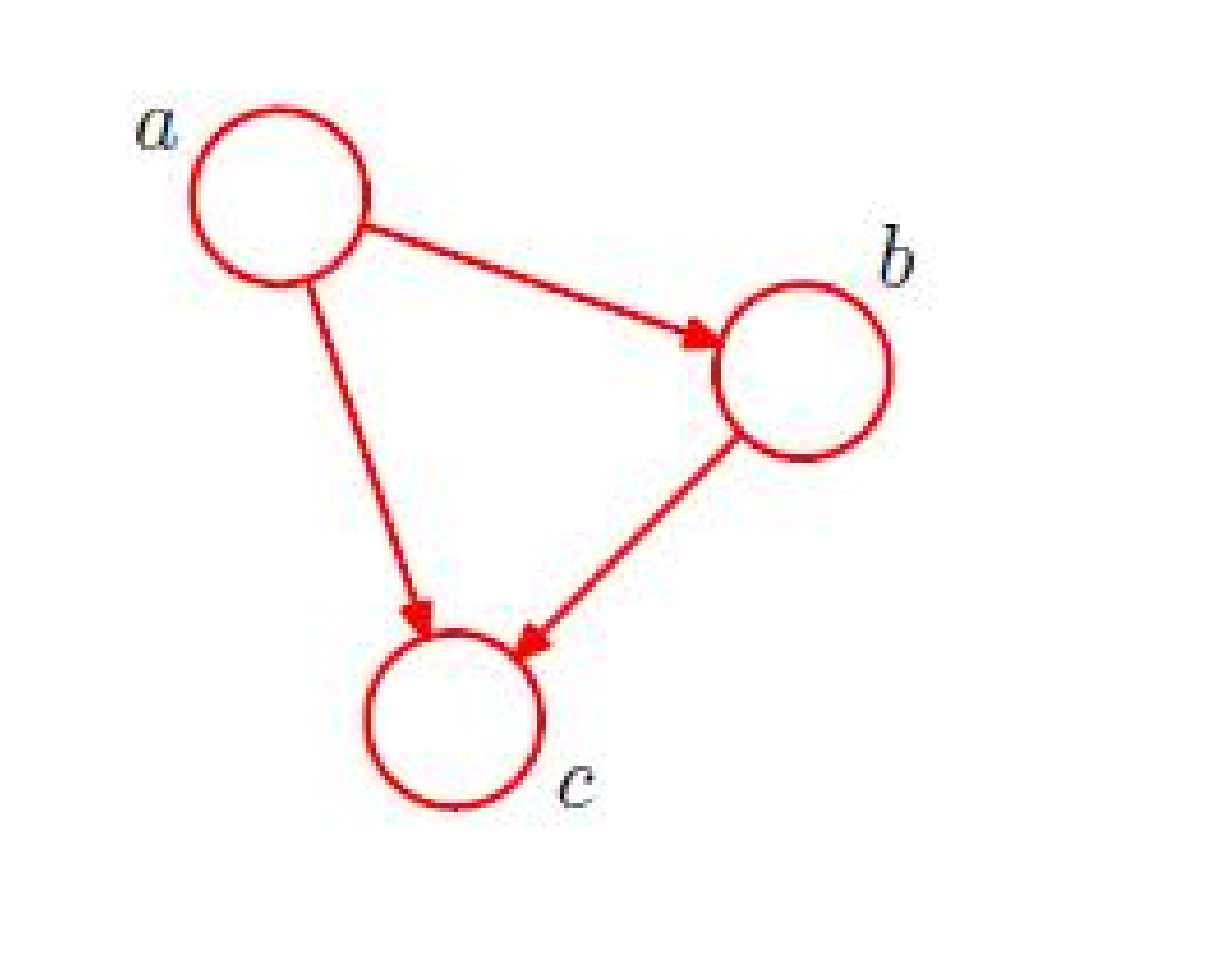
\includegraphics[width=0.5\linewidth]{./imgs/GM1.eps}
    \caption{}
    \label{GM1}
\end{minipage}
\begin{minipage}{0.5\textwidth}
    \centering
    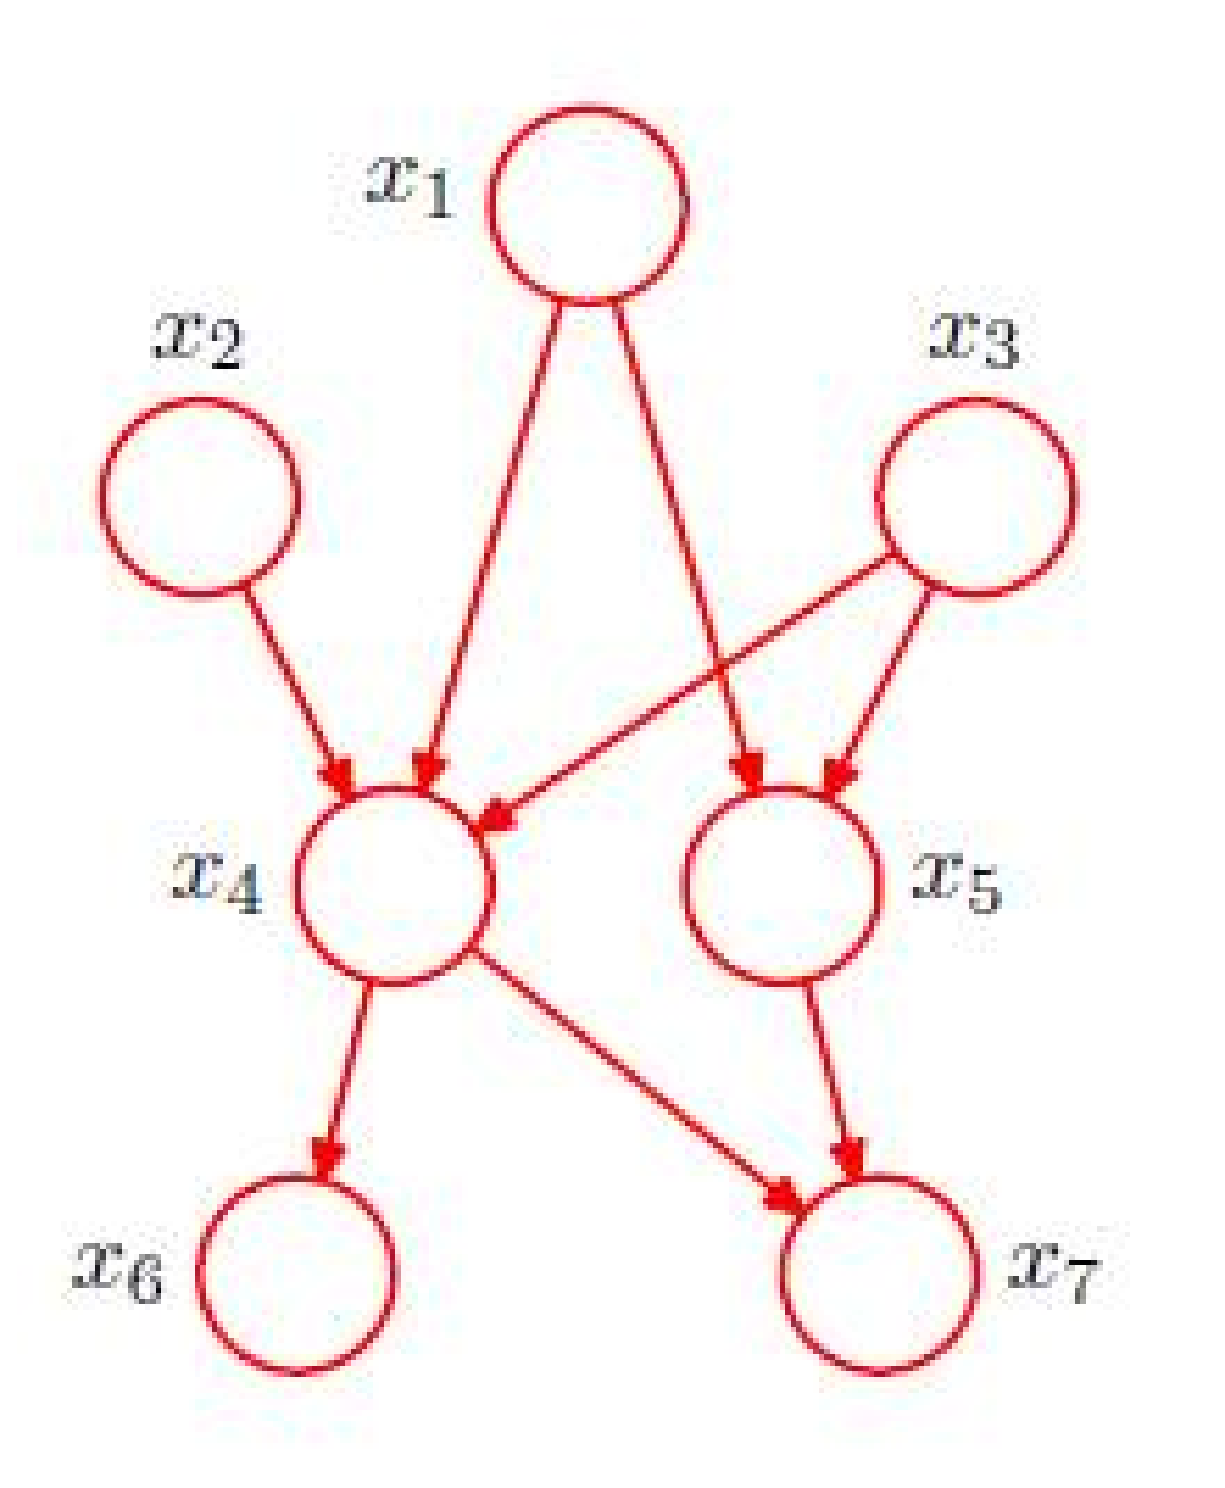
\includegraphics[width=0.5\linewidth]{./imgs/GM2.eps}
    \caption{}
    \label{GM2}
\end{minipage}
\end{figure}
\newline
\textbf{Rule}: for each conditional distribution we add directed links (arrows) to the graph from the nodes corresponding to the variables on which the distribution is conditioned.
\newline
we can extend the decomposition to $K$ variables:
\begin{equation}
    p(x_1,...,x_K) = p(x_K|x_1,...,x_{K-1})...p(x_2|x_1)p(x_1).
    \label{eq8.2}
\end{equation}
And the corresponding directed graph is called \textit{fully connected} because there is a link between every pair of nodes.
\newline
\textbf{Case} Given a directed graph as seen in \ref{GM2}, we can write the corresponding probability product:
\begin{equation}
    p(x_1)p(x_2)p(x_3)p(x_4|x_1,x_2,x_3)p(x_5|x_2,x_3)p(x_6|x_4)p(x_7|x_4,x_5)
    \label{8.3}
\end{equation}
\textbf{Rule}:
\begin{equation}
p(\textbf{x}) = \Pi_{k=1}^Kp(x_k|\mathrm{pa}_k)
\label{8.4}
\end{equation}
where $\mathrm{pa}_k$ denotes the set of parents of $x_k$, and $\textbf{x} = \{x_1,..,x_K\}$.
\newline
The directed graphs that we are considering are subject to an important restriction namely that there must be no \textit{directed cycles}, in other words there are no closed paths within the graph such that we can move from node to node along links following the direction of the arrows and end up back at the starting node. Such graphs are also called \textit{directed acyclic graphs}, or \textit{DAGs}. This is equivalent to the statement that there exists an ordering of the nodes such that there are no links that go from any node to any lower numbered node.
\subsubsection{Example: polynomial regression}
For more complex models, we shall adopt the convention that random variables will be denoted by open circles, and deterministic parameters will be denoted by smaller solid circles.
some concepts: \textit{observed variables, hidden variables, deterministic parameters}.
\subsubsection{Generative models}
\textit{sampling}: given a joint distribution, we want to draw a sample $\hat x_1, \hat x_2, ..., \hat x_K$ from it.
\textbf{ancestral sampling}
\newline
We start with the lowest-numbered node and draw a sample from the distribution $p(x_1)$, which we all $\hat x_1$. Then we work through each of the nodes in order, so that for node n we draw a sample from the conditional distribution p(xn|pan)
in which the parent variables have been set to their sampled values. Note that at each stage, these parent values will always be available because they correspond to lower-numbered
nodes that have already been sampled. The graphical model captures the \textit{causal} process by which the observed data was generated. For this reason, such models are often called \textit{generative} models. But the regression problem is not generative because there is no probability distribution associated with the input variable $x$, and it is not possible to generate synthetic data points from this model. But we can make it generative by introducing a suitable prior distribution $p(x)$, at the expense of a more complex model.
\subsubsection{Discrete variables}
\textit{parent-child pair in a directed graph. Two cases are particularly worthy of note, namely when the parent and child node each correspond to discrete variables and when they each correspond to Gaussian variables, because in these two cases the relationship can be extended hierarchically to construct arbitrarily complex directed acyclic graphs.}
\newline
\textbf{Case}:  discrete variable $\textbf{x}$ having $K$ possible states is given by
\begin{equation}\label{eq8.5}
  p(\bf{x}|\bf{mu}) =  \Pi_{k=1}^K\mu_k^{x_k}
\end{equation} governed by $\bf{\mu}$.
Suppose we have to discrete variables $\bf x_1, \bf x_2$, joint distribution can be written as
\begin{equation}\label{eq8.6}
  p(\bf x_1, \bf x_2|\bf{\mu})=\Pi_{k=1}^K\Pi_{k=1}^K\mu_{kl}^{x_{1k}x_{2l}}.
\end{equation}
$x_{1k}$ denotes the $k^{th}$ component of $\bf x_1$.
\newline
$K^2-1$ parameters. If we have $M$ variables, there is $K^M-1$ parameters, exponential with the num $M$.
\newline
Suppose $\bf x_1$ and $\bf x_2$ are independent. Each variable is then described by a separate multinomial distribution, and total number of parameters will be $2(K-1)$. If extend to $M$ variables, there will be $M(K-1)$ variables, linear growth.
\newline
\textbf{Generally case}: more links than independent variables but less links than a fully connected graph.
\newline
We can turn a graph over discrete variables into a Bayesian model by introducing Dirichlet priors for the parameters.
\newline
Another way of controlling the exponential growth in the number of parameters
in models of discrete variables is to use parameterized models for the conditional
distributions instead of complete tables of conditional probability values.
\subsubsection{Linear-Gaussian models}

\subsection{Conditional Independence}
If
\begin{equation}\label{eq8.7}
  p(a|b, c) = p(a|c),
\end{equation}
we say that $a$ is conditionally independent of $b$ given $c$, and we denote this by $$a\ci b|c .$$  And we will have
\begin{equation}\label{eq8.8}
  p(a,b|c) = p(a|c)p(b|c).
\end{equation}
\subsubsection{Examples}
Three examples related to conditional independence: \textit{tail-to-tail, head-to-tail, head-to-head}.
\subsubsection{D-separation}
We wish to ascertain whether a particular conditional
independence statement$$A\ci B |C$$is implied by a given directed acyclic graph.
\newline
i.i.d data points. Given $\mu$, we can say the data points $x_1,x_2,...,x_N$ are conditionally independent, but we can not say the data points are independent. because given $x_1$, the probability of $\mu$ will be affected and then $x_2$ will be affected.
\newline
\textbf{naive Bayes Model} Observation of $\bf{z}$ will block the path between $x_i$ and $x_j$ for $j\neq i$. So, if we are given a training set will, comprising inputs $\{x_1,...,x_N\}$ together with their labels, then we can fit the naive Bayes model to the training data using maximum likelihood assuming that the data are drawn independently from the model.
\newline
We can view a directed graph as a filter and all probability distribution $p(\bf x)$ that will be allowed through can make a set $\mathcal {DF}$.
\newline
\textbf{Markov blanket}.
\begin{equation}\label{eq8.9}
  p(\bf{x}_i|\bf{x}_{\{j\neq i\}}) = \frac{p(\bf x_1,...\bf x_D)}{\int p(\bf x_1,...,\bf x_D)\rm d\bf x_i}=\frac{\prod_k p(\bf x_k|\rm{pa}_k)}{\int \prod_k p(\bf x_k|\rm{pa}_k)\rm{d}\bf x_i}
\end{equation}
Some factors in $\prod_k p(\bf x_k|\rm{pa}_k)$ will disappear if they are not relative to $\bf x_i$.
\subsection{Markov Random Fields}
A \textit{Markov random field}, also known as a \textit{Markov network} or an \textit{undirected graphical model} , has a set of nodes each of which corresponds to a variable or group of variables, as well as a set of links each of which connects a pair of nodes. The links are undirected, that is they do not carry arrows.
\subsubsection{Conditional independence properties}
Properties in an undirected graph is much simpler than those in a directed graph because the nodes linked in a pair is symmetric, and there is no head-to-head situation. So if all paths that connect nodes in $A$ to nodes in $B$ pass through one or more nodes in the set $C$, then all such paths are 'blocked' and so the conditional independence property hold, aka. $$A\ci B|C$$.
\subsubsection{Factorization properties}
If two nodes are not linked directly, then we can obtain
\begin{equation}\label{eq8.10}
  p(x_i,x_j|\bf{x}_{\backslash\{i,j\}}) = p(x_i|\bf x_{\backslash\{i,j\}})p(x_j|\bf x_{\backslash\{i,j\}})
\end{equation}
\textbf{clique}:a subset of nodes in a graph such that there exists a link between all pairs of nodes in the subset. \newline
\textbf{maximal clique}:a clique such that it is not possible to include any
other nodes from the graph in the set without it ceasing to be a clique.\newline
Denote a clique by $C$ and the set of variables in that clique by $\bf x_C$. Then the joint distribution is written as a product of \textit{potential functions}
$\phi_C(\bf x_C)$ over maximal cliques of the graph
\begin{equation}\label{eq8.11}
  p(\bf x) = \frac{1}{Z}\prod_{C}\phi_C(\bf x_C).
\end{equation}
Here the quantity Z, sometimes called the partition function, is a normalization constant
and is given by
\begin{equation}\label{eq8.12}
  Z=\sum_{X}\prod_{C}\phi_C(\bf x_C)
\end{equation}
\textit{energy function} $E(\bf x_C)$
\begin{equation}\label{eq8.13}
  \phi_C(\bf x_C) = \exp\{-E(\bf x_C\}
\end{equation}
\subsubsection{Relation to directed graphs}
\begin{figure}
  \centering
  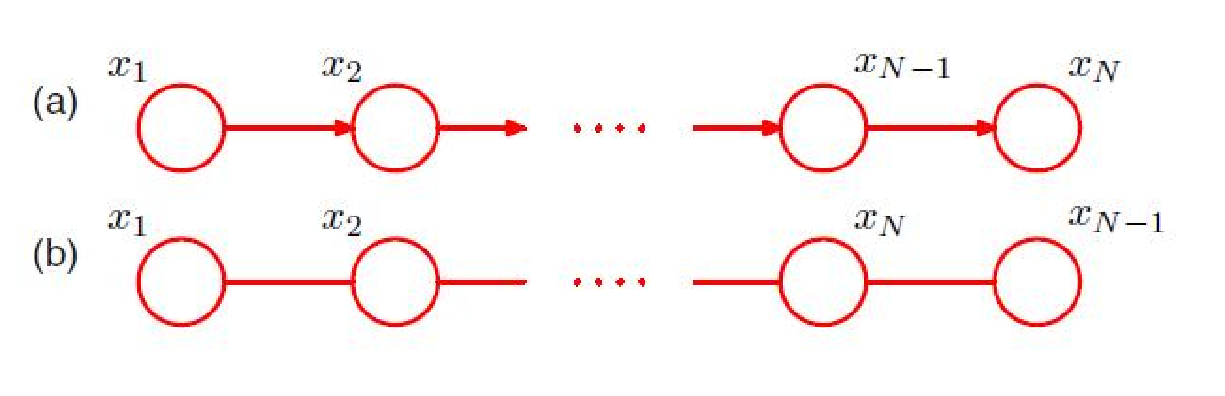
\includegraphics[width=\textwidth]{./imgs/GM3.eps}
  \caption{}\label{GM3}
\end{figure}
Given a directed graph as a chain shown in figure\ref{GM3}(a).
\begin{equation}\label{eq8.14}
  p(\bf x) =p(x_1)p(x_2|x_1)p(x_3|x_2)...p(x_N|x_{N-1})
\end{equation}
Also, for undirected graph shown in figure\ref{GM3}(b).
\begin{equation}\label{eq8.15}
  p(\bf x) = \frac{1}{Z}\psi_{1,2}(x_1,x_2)\psi_{2,3}(x_2,x_3)...\psi_{N-1,N}(x_{N-1},x_N).
\end{equation}
And we define
\begin{align}\label{eq8.15}
  \psi_{1,2}(x_1,x_2) = p(x_1)p(x_2|x_1) \\
  \psi_{2,3}(x_2,x_3)=p(x_3|x_2) \\
  \vdots \\
  \psi_{N-1,N}(x_{N-1},x_N) = p(x_N|x_{N-1})
\end{align}

\section{Continuous Latent Variables}
The simplest continuous latent variable model assumes Gaussian distributions
for both the latent and observed variables and makes use of a linear,Gaussian dependence of the observed variables on Ihe slate of the latent variables. This leads
to a probabilistic formulation of the well-known technique of principal component
analysis (PCA), as well as to a related model called factor analysis.
\subsection{Principal Component Analysis}
Two commonly used definitions of PCA:
\begin{itemize}
  \item the orthogonal projection of the data onto a lower dimensional linear space.
  \item the linear projection that minimizes the average projection cost.
\end{itemize}
\subsubsection*{Maximum variance formulation}
Consider a data set of observations $\{\mrm x_n\}$ and $\mrm x_n$ is a Euclidean variable with dimensionality $D$. Our goal is to project the data onto a space having dimensionality $M<D$ while maximizing the variance of the projected data.

To begin with, we consider $M=1$ and we define the one-dimensional space using a $D-$dimensional vector $\mrm u_1$, which is a unit vector. So the mean of the projected data is $\mrm u_1\bar{\mrm x}$ where
\begin{equation}\label{}
  \bar{\mrm x}=\frac1N\sum_{n=1}^{N}\mrm x_n
\end{equation}
And the variance of the projected data is given by
\begin{equation}\label{}
  \frac1N\sum_{n=1}^{N}\{\mrm u_1^T\mrm x_n-\mrm u_1^T\bar{\mrm x}\}^2 = \mrm (u_1^TSu_1)
\end{equation}
where $\mrm S$ is the data covariance matrix2de defined by
\begin{equation}\label{}
  J(\mrm u_1) = \mrm S=\frac1N\sum_{n=1}^{N}(\mx _n-\bar{\mx})(\mx_n-\bar\mx)^T
\end{equation}

Then we maximize the $J(\mrm u_1)$ with respect to $\mrm u_1$ under the constraint $\mrm u_1^T\mrm u_1 = 1$ and we obtain
\begin{equation}\label{}
  \mrm S\mrm u_1=\lambda_1\mrm u_1
\end{equation}
which says that $\mrm u_1$ must be an eigenvector of $\mrm S$. And
\begin{equation}\label{}
  \mrm{u_1^TSu}=\lambda_1,
\end{equation}
so we will choose $\mrm u_1$ to be the eigenvector corresponding to the largest eigenvalue.

\subsubsection*{Minimum-error formulation}
Now we discuss another formulation of PCA based on projection error minimization. To do this, we introduce a complete orthogonal set of $D-$dimensional basis vectors $\{\mrm u_1\}$ that satisfies
\begin{equation}\label{}
  \mrm{u^T_iu_j} = \delta_{ij}.
\end{equation}
And each data point can be represented by a linear combination of the basis vectors
\begin{equation}\label{}
  \mx_n=\sum_{i=1}^{D}\alpha_{ni}\mrm u_i.
\end{equation}
where $\alpha_{ni} = \mx_n^Tu_j$. And if we want to reduce the dimensionality to $M<D$, we can approximate each data point $\mx_n$ by
\begin{equation}\label{}
  \tilde{\mx_n} = \sum_{i=1}^{M}z_{ni}\mrm u_i+\sum_{i=M+1}^{D}bi\mrm u_i
\end{equation}
where $z_{ni}$ depend on the particular point while $b_i$ is fixed for all points. Then we define the loss by
\begin{equation}\label{}
  J=\frac{1}{N}\sum_{n=1}^{N}\|\mx_n-\tilde{\mx_n}\|^2.
\end{equation}
Then we minimize $J$ by setting the derivatives with respect to $\{z_{nj}\}$ and $b_i$ to zero, and we obtain
\begin{gather}\label{}
  z_{nj} =  \mx_n^T\mrm u_j \\
  b_j = \bar{\mx}^T\mrm u_j.
\end{gather}
So the distortion is
\begin{equation}\label{}
  \mx_n-\tilde{\mx}_n = \sum_{i=M+1}^{D}\{(\mx_n-\bar{\mx}_n)^T\mrm u_i\}\mrm u_i
\end{equation}
and
\begin{equation}\label{}
  J = \frac{1}{N}\sum_{n=1}^{N}\sum_{i=M+1}^{D}(\mx_n^T\mrm u_i - \bar{\mx}^T\mrm u_i)^2=\sum_{i=M+1}^{D}\mrm u_i^T\mrm S\mrm u_i.
\end{equation}
Then we need to minimize $J$ with respect to $\{\mrm u_i\}$ under constraint $\mrm u_i^T\mrm u_i = 1$ and we can obtain
\begin{equation}\label{}
  \mrm S\mrm u_i = \lambda_i\mrm u_i
\end{equation}
and
\begin{equation}\label{}
  J = \sum_{i=M+1}^{D}\lambda_i.
\end{equation}

\subsubsection*{Application of PCA}
\subsubsection*{PCA for high-dimensional data}
In some situations, $N < D$, a set of $N$ points in $D$-dimensional space defines a linear subspace whose dimensionality is at most $N-1$. So if we perform PCA we will find that at least $D-N+1$ of the eigenvalues are zero, and the time cost is very large. We can solve this problem as follows. Define $\mrm X$ to be the $N\times D$-dimensional centred data matrix, whose $n^{\mrm{th}}$ row is given by $\mx_n-\bar{\mx}^{\mrm T}$. Then $\mrm S = \frac{1}{N}\mrm{X}^T\mrm X$ and
\begin{gather}\label{}
  \frac{1}{N}\mrm X^T\mrm X\mrm u_i=\lambda_i\mrm u_i. \\
  \frac{1}{N}\mrm X\mrm X^T(\mrm X\mrm u_i) = \lambda_i(\mrm X\mrm u_i) \\
  \frac{1}{N}\mrm X\mrm X^T\mrm v_i = \lambda_i\mrm v_i
\end{gather}
where $\mrm v_i = \mrm X\mrm u_i$. And
\begin{equation}\label{}
  (\frac{1}{N}\mrm X^T\mrm X)(\mrm X^T\mrm v_i) = \lambda_i(\mrm X^T\mrm v_i),
\end{equation}
so $(\mrm X\mrm v_i)$ is an eigenvector of $\mrm S$ with eigenvalue $\lambda_i$.

\subsection{Probabilistic PCA}
Previously we discussed PCA based on a linear projection of the data onto a subspace of lower dimensionality than the original data space. We now show that PCA can also be expressed as the maximum likelihood solution of a probabilistic latent variable model. This reformulation of PCA has several advantages compared with the conventional PCA.\newline
We can formulate probabilistic PCA by first introducing an explicit latent variable $\mbf z$ corresponding to the principal-component subspace. Next we define a Gaussian prior distribution $p(\mbf z)$ with a Gaussian conditional distribution $p(\mbf x|\mbf z)$.
\begin{gather}\label{}
  p(\mbf z) = \normD(\mbf z|\mbf{0}, \mbf I) \\
  p(\mbf x|\mbf z) = \normD(\mbf x|\mbf W\mbf z+\mu, \sigma^2\mbf I)
\end{gather}
In a generative view, the $D$-dimensional observed variable $\mbf x$ is defined by a linear transformation of the $M$-dimensional latent variable $\mbf z$ plus additive Gaussian noise, so that
\begin{equation}\label{}
  \mbf x=\mbf W\mbf z+\mu+\epsilon
\end{equation}
where $\mbf z$ is an $M$-dimensional Gaussian latent variable and $\epsilon$ is a $D$-dimensional zero-mean Gaussian-distributed noise variable with covariance $\sigma^2\mbf I$. So, the reverse the mapping, from data space to latent space, will be obtained shortly using Bayes' theorem. Now we want to determine the values of $\mbf W, \mu,\sigma^2$ using maximum likelihood.
\begin{equation}\label{}
  p(\mbf x) = \int p(\mbf x|\mbf z)p(\mbf z)\mrm d\mbf z) = \normD(\mbf x|\mu, \mbf C),
\end{equation}
where
\begin{equation}\label{}
  \mbf C = \mbf W\mbf W^T+\sigma^2\mbf I
\end{equation}
Note that if we define $\tilde{\mbf W} = \mbf {WR}$ where $\mbf R$ is orthogonal, then $\tilde{\mbf W}\tilde{\mbf W}^T=\mbf{WW}^T$
\begin{equation}\label{}
  \mbf C^{-1} = \sigma^{-1}\mbf I-\sigma^{-2}\mbf W\mbf M^{-1}\mbf W^T,
\end{equation}
where $\mbf M\in \mathbb{R}^{M\times M}$ and $\mbf M=\mbf W^T\mbf W$, reducing computing cost by changing reversing $\mbf C$ to reversing $\mbf M$. \newline
So,
\begin{equation}\label{}
  p(\mbf z|\mbf x) = \normD(\mbf z|\mbf M^{-1}\mbf W^T(\mbf x-\mu),\sigma^{-2}\mbf M)
\end{equation}
where the mean is related to $\mbf x$ while covariance is not.
\subsubsection*{Maximum likelihood}
Given a data set $\mbf X=\{\mbf x_n\}$, then,
\begin{equation}\label{}
  \ln p(\mbf X|\mu,\mbf W,\sigma^2) = \sum_{n=1}^{N}\ln p(\mbf x_n|\mbf W,\mu,\sigma^2)=-\frac{ND}{2}\ln(2\pi)-\frac{N}{2}\ln|\mbf C|-\frac{1}{2}\sum_{n=1}^{N}(\mbf x_n-\mu)^T\mbf C^{-1}(\mbf x_n-\mu)
\end{equation}
and we obtain
\begin{gather}\label{PCA.1}
  \mu_{\mrm{ML}} = \bar{\mbf x}=\frac{1}{N}\sum_{n=1}^{N}\mbf x_n \\
  \ln p(\mbf x|\mbf W,\mu,\sigma^2) = -\frac{N}{2}\{D\ln(2\pi)+\ln|\mbf C|+\mrm{Tr}(\mbf C^{-1}\mbf S)\}
\end{gather}
where $\mbf S = \frac{1}{N}\sum_{n=1}^{N}(\mbf x_n-\bar{\mbf x})(\mbf x_n-\bar{\mbf x})^T$. Maximizing with respect to $\mbf W$ and $\sigma^2$, we find that all stationary points satisfy
\begin{equation}\label{}
  \mbf W_{\mrm{ML}} = \mbf U_M(\mbf L_M-\sigma^2\mbf I)^{1/2}\mbf R
\end{equation}
where $\mbf U_M\in \mathbb{R}^{D\times M}$ with columns choosing from the eigenvectors $\mbf v_i$ of $\mbf S$, $\mbf L_M$ offers the eigenvalues $\lambda_i$, and $\mbf R$ is any orthogonal matrix. And maximum is reached when we choose the most largest $M$ eigenvalues and their corresponding eigenvectors. Then corresponding value for $\sigma^2$ is
\begin{equation}\label{}
  \sigma^2_{\mrm{ML}} = \frac{1}{D-M}\sum_{i=M+1}^{D}\lambda_i
\end{equation}
which is unchanged by rotation in the latent variable. \newline
For $\mbf C=\mbf W\mbf W^T+\sigma^2\mbf I$, on direction $\mbf v, \mbf v^T\mbf v = 1$, if $\mbf v$ is orthogonal to the subspace, which is shown as $\mbf v^T\mbf U=0$, then $\mbf v^\mbf C \mbf v = \mbf v^T\mbf {WW}^T\mbf v+\sigma^2\mbf v^T\mbf v = \sigma^2$, in which, we omitted $\mbf W^T\mbf v = \mbf R^T[(\mbf L_M-\sigma^2\mbf I)^{1/2}]^T\mbf U_M\mbf v = 0$. \newline
If $\vv = \uu_i\in \mathbb{R}^D$, is an eigenvector, then $\vv^T\WW\WW^T\vv=\lambda_i$.\newline
If we choose $M=D$, no reduction will be achieved and $\UU_M=\UU, \mbf L_M=\mbf L, \SS=\UU\mbf L\UU^T$, therefore, $\CC = \mbf S$. \newline
Probabilistic PCA is most natural expressed as a mapping from the latent space into the data space $\xx=\WW\xx+\mu+\epsilon$.
\subsubsection*{EM algorithm for PCA}
In very high dimensional space, although there is close-formed solution for PCA, the computing is very time-consuming, so we turn to using EM algorithm to so PCA to reduce the time costing. \newline
We write down the complete-data log likelihood and take its expectation with respect to the posterior distribution of the latent distribution evaluated using 'old' parameter values. Maximization of this expected comple-data likelihood then yields the 'new' ;parameter values.
\begin{equation}\label{}
  \ln p(\XX,\ZZ|\mu, \WW,\sigma^2) = \sum_{n=1}^{N}\{\ln p(\xx_n|\zz_n)+\ln p(\zz_n)\}
\end{equation}
where the $\mrm n^{\mrm{th}}$ row of the matrix $\ZZ$ is given by $\zz_n$. We can compute $\mu_{\mrm{ML}}$ using \ref{PCA.1} and it is convenient to substitute for $\mu$ at this stage.
\begin{align}\label{}
  \mathbb{E} [\ln p(\XX,\ZZ|\mu,\WW,\sigma^2)] & = -\frac{n=1}{N}\{\frac{D}{2}\ln(2\pi\sigma^2)+\frac12\mrm{Tr}(\mathbb{E}[\zz_n\zz_n^T]) \\
  & +\frac{1}{2\sigma^2}\|\xx_n-\mu\|^2-\frac{1}{\sigma^2}\mathbb{E}[\zz_n]^T\WW^T(\xx_n-\mu) \\
  & + \frac{1}{2\sigma^2}\mrm{Tr}(\mathbb{E}[\zz_n\zz_n^T]\WW^T\WW)\}
\end{align}\label{}
\begin{gather}\label{}
  \mathbb{E}[\zz_n] = \MM^{-1}\WW^T(\xx_n-\bar{\xx}) \\
  \bb{E}[\zz_n\zz_n^T] = \sigma^2\MM^{-1}+\bb{E}[\zz_n]\bb{E}[\zz_n]^T
\end{gather}
where $\MM = \WW^T\WW+\sigma^2\II$.
In the M step, we maximize with respect to $\WW$ and $\sigma^2$, keeping the posterior statistics fixed. Maximization with respect to $\sigma^2$ is straightforward, and
\begin{gather}\label{}
  \WW_{\mrm{new}} = [\sum_{n=1}^{N}(\xx_n-\bar{\xx})\bb{E}[\zz_n]^T][\sum_{n=1}^{N}\Exp[\zz_n\zz_n^T]]^{-1}  \\
  \sigma^2_{\mrm{new}} = \frac{1}{ND}\sum_{n=1}^{N}\{\|\xx_n-\bar{\xx}\|^2-2\Exp[\zz_n]^T\WW_{\mrm{new}}^T(\xx_n-\bar{\xx})+\mrm{Tr}(\Exp[\zz_n\zz_n^T]\WW_{\mrm{new}}^T\WW_{\mrm{new}}) \}
\end{gather}
\subsubsection*{Bayesian PCA}
\subsubsection*{Factor analysis}
The only difference between FA and PCA is that we assume
\begin{equation}\label{}
  p(\xx|\zz) = \normD(\xx|\WW\zz+\mu,\Psi)
\end{equation}
in FA, where $\Psi$ is diagonal. Now, the marginal distribution of $\xx$ is $p(\xx) = \normD(\xx|\mu, \CC), \CC = \WW\WW^T+\Psi$. When we do maximum likelihood, $\mu_{\mrm{ML}}$ is still the sample mean, while there is no close-formed solution for $\WW$ and we must turn to EM algorithm. And here, the sufficient  statistics are
\begin{gather}\label{}
  \Exp[\zz_n] = \mbf G\WW^T\Psi^{-1}(\xx_n-\bar \xx) \\
  \Exp[\zz_n\zz_n^T] = \mbf G+\Exp[\zz_n]\Exp^T[\zz_n] \\
\end{gather}
where $\mbf G = (\II+\WW^T\Psi\rev\WW)\rev$.

\subsection{Kernel PCA}
In this section, we will apply the technique of kernel to PCA.\newline
Suppose we have a data set of $N$ observations $\{\xx_n\}$ and $\sum_{n=1}^{N}\xx_n$, $\mbf S=\frac{1}{N}\sum_{n=1}^{N}\xx_n\xx_n^T$ \newline
\begin{equation}\label{}
  \mbf S\uu_i=\lambda_i\uu_i, \uu_i^T\uu_i = 1.
\end{equation}
Now consider a nonlinear transformation $\phi(\xx)$ into an $M$-dimensional feature space, so that each data point $\xx_n$ is thereby projected onto a point $\phi(\xx_n)$.
For the moment, let us assume that the projected data set also has zero mean, so that $\sum_{n=1}^{N}\phi(\xx_n) = \mbf 0$. The $M\times M$ sample covariance matrix in feature space is given by
\begin{equation}\label{}
  \CC = \frac{1}{N}\sum_{n=1}^{N}\phi(\xx_n)\phi(\xx_n)^T
\end{equation}
and its eigenvectors is defined by
\begin{equation}\label{}
  \CC\vv_i=\lambda_i\vv_i,\ \vv_i^\mrm{T}\vv_j=\delta_{ij}
\end{equation}
$i=1, \dots, M$. We want to solve the eigenvalue problem without having to work explicitly in the feature space. For the definition of $\CC$, the eigenvectors $\vv_i$ satisfies
\begin{equation}\label{}
  \frac{1}{N}\sum_{n=1}^{N}\phi(\xx_n)\{\phi(\xx_n)^T\vv_i\} = \lambda_i\vv_i
\end{equation}
and we see (provided $\lambda_i>0$) that the vector $\vv_i$ is given by a linear combination of the $\phi(\xx_n)$ and so can be written in the form
\begin{equation}\label{}
  \vv_i=\sum_{n=1}^{N}a_{in}\phi(\xx_n).
\end{equation}
Substituting this expansion back into the eigenvector equation, we obtain
\begin{equation}\label{}
  \frac1N\sum_{n=1}^{N}\phi(\xx_n)\phi(\xx_n)^T\sum_{m=1}^{N}a_{im}\phi(\xx_m) = \lambda_i\sum_{n=1}^{N}a_{in}\phi(\xx_n).
\end{equation}
Multiply both sides by $\phi(\xx_l)^T$ and we obtain
\begin{equation}\label{}
  \frac1N\sum_{n=1}^{N}k(\xx_l,\xx_n)\sum_{m=1}^{N}a_{im}k(\xx_n,\xx_m) = \lambda_i\sum_{n=1}^{N}a_{in}k(\xx_l,\xx_n).
\end{equation}
This can be written in matrix notation as
\begin{equation}\label{}
    \KK^2\mbf a_i=\lambda_iN\KK\mbf a_i
\end{equation}
where $\mbf a_i$ is an $N$-dimensional column vector with elements $a_{ni}$ for $n = 1, \dots, N$. We can find solutions for $\mbf a_i$ by solving:
\begin{equation}\label{}
    \KK\mbf a_i = \lambda_iN\mbf a_i.
\end{equation}
We require the eigenvectors in feature space be normalized.
\begin{equation}\label{}
  \vv_i^T\vv_i=\sum_{n=1}^{N}\sum_{m=1}^{N}a_{in}a_{im}\phi(\xx_n)^T\phi(\xx_m) =\mbf a_i\KK\mbf a_i = \lambda_iN\mbf a_i^T\mbf a_i.
\end{equation}
Then the projection of a point $\xx$ onto the eigenvector $i$ is given by
\begin{equation}\label{}
  y_i(\xx) = \phi(\xx)^T\vv_i=\sum_{n=1}^{N}a_{in}\phi(\xx)^T\phi(\xx_n) = \sum_{n=1}^{N}a_{in}k(\xx,\xx_n).
\end{equation}
The dimension $M$ of the feature space can be much larger than $D$ and thus we can find a number of nonlinear principal components that can exceed $D$. However, the number of nonzero eigenvalues cannot exceed the number $N$ of data points.

\subsection{Nonlinear Latent Variable Methods}

\section{FOR NEW}


\chapter{Algorithms}
\section{Nonparametric Methods}
In probability theory, we have  focussed on the use of probability distributions
having specific functional forms governed by a small number of parameters whose
values are to be determined from a data set.\textbf{This is called the parametric approach}.
\textbf{to density modelling}\newline
\textbf{histogram}
$$p_i = \frac{n_i}{N\Delta_i}=\frac{n_i}{N\Delta}$$
how to choose proper $\Delta$ is very important and sensitive
\subsection{Kernel density estimators}
Consider some small region $\mathcal R$ containing $\mathrm x$, the probability mass is given by
$$P=\int_{\mathcal R}p(\mathrm x)\mathrm {dx}$$
N observations drawn from $p(\mathrm x)$ \newline
Total number $K$ of points that lie inside $\mathcal R$ will be distributed according to the binomial distribution.
$$\mathrm {Bin}(K|N,P) =$$
so mean faction in the region will be $\mathrm E[K/N] = P$, and $\mathrm {var}[K/N] = P(1-P)/N$.\newline
$P=p(\mathrm x)V$ if $\mathcal R$ is small enough, so $p(\mathrm x) = \frac{K}{NV}$\newline
\textbf{based on two contradictory assumptions}: region is sufficiently small that the density is approximately constant over the region and yet sufficiently large that the number $K$ of points falling inside the region is sufficient for the binomial distribution to be sharply peaked.\newline
If we fix $V$ and determine $K$ from the data,  giving rise to the kernel approach.
$k(\mathrm u) =1$ if $|u_i|\leq 1/2, i=1, 2, \dots, D, $ else $0$ .\newline
This represents a unit cube centred on the origin. The function $k(\mathrm u)$ is an example of a \textit{kernel function}\newline
So $$K = \sum_{n=1}^Nk(\frac{\mathrm x-\mathrm x_n}{h}), p(\mathrm x) = \frac1N\sum_{n=1}^N\frac1{h^D}k(\frac{\mathrm x-\mathrm x_n}{h})$$
and common choice for a kernel is Gaussian, which give rise to the following kernel density model:
$$p(\mathrm x) = \frac1N\sum_{n=1}^N\frac{1}{(2\pi h^2)^{1/2}}\exp\{-\frac{||\mathrm x-\mathrm x_n||^2}{2h^2}\}$$
also a trade-off between sensitivity to noise at small $h$ and over-smoothing at large $h$\newline
computational cost.
\subsection{Nearest-neighbour methods}
idea: allow the radius of the sphere to grow until it contains precisely $K$ data points, then the volume of the sphere is set to $V$.\newline
K-nearest-neighbour technique for density estimation can be extended to classification.
$N_k$ points in class $\mathcal C_k$, $\sum_kN_k=N$
\newline
If we want to classify a new point $\mathrm x$, we draw a sphere centred on $\mathrm x$ containing precisely $K$ points. Suppose this sphere contains $K_k$ points from $\mathcal C_k$. Then
$$p(\mathrm x|\mathcal C_k) = \frac{K_k}{N_kV} , p(\mathrm x) = \frac{K}{NV}, p(\mathcal C_k) = \frac{N_k}{N}$$
so $p(\mathcal C_k|\mathrm x) = \frac{K_k}{K}$
\section{Inference Algorithms in Graphical Models}
\subsection{Inference on a chain}
Consider the graph shown in figure\ref{GM3}. The joint distribution for this graph takes the form
\begin{equation}\label{eq8.16}
  p(\bf x) = \frac{1}{Z}\psi_{1,2}(x_1,x_2)\psi_{2,3}(x_2,x_3)...\psi_{N-1,N}(x_{N-1},x_N).
\end{equation}
If we want to get marginal distribution $p(x_n)$ for a specific node, we should sum the joint distribution over all variables except $x_n$, so that
\begin{equation}\label{eq8.17}
  p(x_n) = \sum_{x_1}...\sum_{x_{n-1}}\sum_{x_{n+1}}...\sum_{x_N}p(\bf x)
\end{equation}
But this way will cost so much computational resources, so we want to find another simpler way:
\begin{align}\label{eq8.18}
  p(x_n) =  & \frac{1}{Z}[\sum_{x_{n-1}}\psi_{n-1,n}(x_{n-1},x_n)\dots[\sum_{x_2}\psi_{2,3}(x_2,x_3)[\sum_{x_1}\psi_{1,2}(x_1,x_2)]]\dots] \\
   & [\sum_{x_{n+1}}\psi_{n,n+1}(x_n,x_{n+1})\dots[\sum_{x_N}]\psi_{N-1,N}(x_{N-1},x_{N})]\dots]  \\
   = & \frac{1}{Z}\mu_{\alpha}(x_n)\mu_{\beta}(x_n)
\end{align}
As shown in figure\ref{GM4}, we can see message passed in the chain and we can compute $\mu_{\alpha}(x_i)$ and $\mu_{\beta}(x_i)$ recursively for any $i=1, 2, \dots, N$.
\begin{equation}\label{eq8.19}
  \mu_{\alpha}(x_n) = \sum_{x_{n-1}}\psi_{n-1,n}(x_{n-1},x_n)\mu_{\alpha}(x_{n-1}).
\end{equation}
and
\begin{equation}\label{eq8.20}
  \mu_{\alpha}(x_2) = \sum_{x_1}\psi_{1,2}(x_1,x_2).
\end{equation}
Similar for $\mu_{\beta}(x_n)$
\begin{figure}[bth]
  \centering
  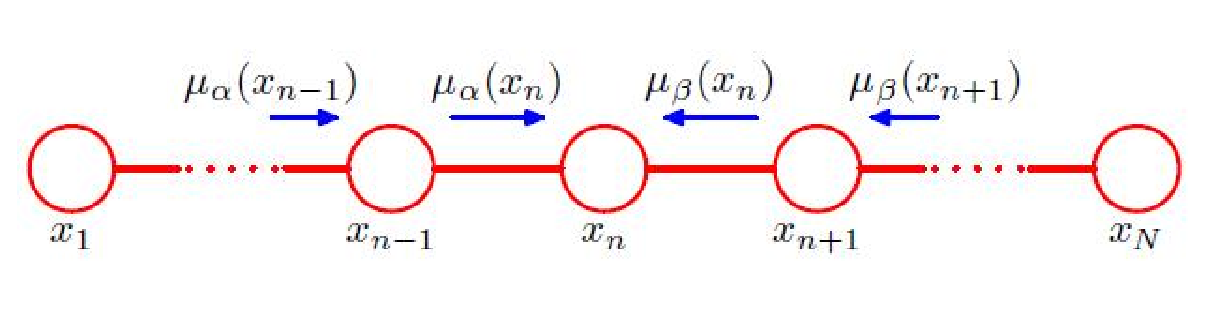
\includegraphics[width=\textwidth]{./imgs/GM4.eps}
  \label{GM4}
\end{figure}
\subsection{Inference on a tree: sum-product algorithm}
Tree do not have loops.
\subsubsection{factor graphs}
In a factor graph, there is a node (depicted as usual by \textbf{a circle}) for every variable
in the distribution, as was the case for directed and undirected graphs. There are also
additional nodes (depicted by \textbf{small squares}) for each factor fs(xs) in the joint distribution.\newline
For example,
\begin{equation}\label{eq8.21}
  p(\bf{x}) = f_a(x_1,x_2)f_b(x_1,x_2)f_c(x_2,x_3)f_d(x_3)
\end{equation}
can be expressed by the factor graph shown in figure\ref{GM5}
\begin{figure}
  \centering
  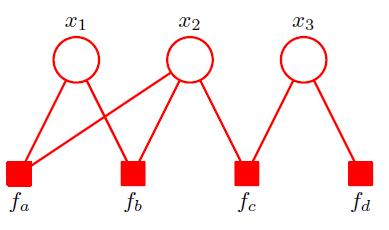
\includegraphics[width=0.5\textwidth]{./imgs/GM5.jpg}
  \caption{Example of a factor graph}\label{GM5}
\end{figure}
Factor graphs are said to be bipartite because they consist of two distinct kinds
of nodes, and all links go between nodes of opposite type.
\subsubsection{sum-product algorithm}
We shall now make use of the factor graph framework to derive a powerful class
of efficient, exact inference algorithms that are applicable to tree-structured graphs.
Here we shall focus on the problem of evaluating local marginals over nodes or
subsets of nodes, which will lead us to the sum-product algorithm.\newline
Our goal is to exploit the structure of
the graph to achieve two things: (i) to obtain an efficient, exact inference algorithm
for finding marginals; (ii) in situations where several marginals are required to allow
computations to be shared efficiently.
\textbf{finding the marginal $p(x)$ for a particular variable node $x$}\newline
$$p(\bf x) = \prod_{s\in ne(x)}F_s(x,X_s)   $$
$$p(x) = \prod_{s\in ne(x)}[\sum_{X_s}F_s(x,X_s)] = \prod_{s\in ne(x)}\mu_{f_s\rightarrow x}(x) $$
$$F_s(x,X_s) =  f_s(x,x_1,...x_M)G_1(x,X_{s1})...G_M(x,X_{sM})$$
$$\mu_{x_m\rightarrow f_s}(x_m) \equiv \sum_{X_{sm}}G_m(x_m,X_{sm})$$
We have therefore introduced two distinct kinds of message, those that go from factor
nodes to variable nodes denoted $\mu_{f\rightarrow x}(x)$, and those that go from variable nodes to
factor nodes denoted $\mu_{x\rightarrow f}(x).$
\textbf{Illustration: example}
\textbf{max-sum algorithm}
Two other common tasks are to find a setting of the variables that has the largest probability
and to find the value of that probability. We therefore seek an efficient algorithm for finding the value of x that maximizes
the joint distribution p(x) and that will allow us to obtain the value of the
joint distribution at its maximum.
\subsection{Exact inference in a general graph}
Goal: deal with graphs having loops.\newline
\textbf{Loopy belief progpagation}
One simple approach to approximate inference in graphs with
loops, which builds directly on the previous discussion of exact inference in trees.
The idea is simply to apply the sum-product algorithm even though there is no guarantee
that it will yield good results. For some graphs, the algorithm will converge, whereas for others it will not. \newline
We will say that a (variable or factor) node a has a message pending on its link to a node b if node a has received any
message on any of its other links since the last time it send a message to b.

\section{Mixture Models and EM}
This section is mainly about chap.9 in \textbf{PRML}.\newline
We can use mixture models to cluster data, as well as build more complex probability distributions. Therefore we begin our discussion of mixture distributions by considering the problem of finding clusters in a set of data points. Then we introduce the latent variable view of mixture distributions in which the discrete variables can be interpreted as defining assignments of data points to specific component of the mixture. Finally we discuss EM in some generality.
\subsection{K-means Clustering}
Suppose we have a data set $\{\mrm x_1,\cdots, \mrm x_N\}$ consisting of $N$ observations of a random $D-$dimensional Euclidean variable $\mrm x$. Our goal is to partition the data set into some number $K$ of clusters.  Firstly we consider a fixed value of $K$. We can formalize this notion by first introducing a set of $D-$dimensional vectors $\mu_k$, where $k=1,\cdots,K$, in which $\mu_k$ is a prototype associated with the $k^{th}$ cluster. For each data point $\mrm x_n$, we introduce a corresponding set of binary indicator variables $r_{nk} \in \{0,1\}$, describing which cluster $\mrm x_n$ is assigned to. We can then define an objective function
\begin{equation}
J = \sum_{n=1}^{N}\sum_{k=1}^{K}r_{nk}\|\mrm x_n-\mu_k\|^2.
\end{equation}
Firstly we choose some initial values for the $\mu_k$. Then in the first phase we minimize $J$ with respect to the $r_{nk}$, keeping the $\mu_k$ fixed. In the second phase we minimize $J$ with respect to the $\mu_k$, keeping $r_{nk}$ fixed. This two-stage optimization is then repeated until convergence. And we obtain
\begin{gather}\label{}
  r_{nk}=\{\begin{matrix}
                 1 & \mrm{if }k=\mrm{arg min_j}\|\mrm x_n-\mu_j\|^2 \\
                 0 & \mrm{otherwise}.
               \end{matrix} \\
  \mu_k = \frac{\sum_nr_{nk}\mrm x_n}{\sum_nr_{nk}}
\end{gather}
A direct implementation of the $K-$means algorithm as discussed here cna be slow because in each E step it is necessary to compute the Euclidean distance between every prototype vector and every data point. Various schemes have been proposed for speeding up this algorithm.


\subsection{Mixtures of Gaussians}
Recall from previous chapter the Gaussian mixture distribution can be written as linear superposition of Gaussians  in the form
\begin{equation}\label{}
  p(\mbf x) = \sum_{k=1}^{K}\pi_k\normD(\mbf x|\mu_k,\Sigma_k).
\end{equation}
Then we can introduce a $K-$dimensional binary random variable $\mbf z$ having a 1-of-$K$ representation in which a particular element $z_k$ is equal to 1 and all other elements are equal to 0. So $z_k \in \{0,1\}$, $\sum_{k}z_k=1$, and $p(z_k=1)=\pi_k$. So
\begin{equation}\label{}
  p(\mrm z) = \prod_{k=1}^{K}\pi_k^{z_k}.
\end{equation}
Similarly, the conditional distribution of $\mrm x$ given a particular value for $\mrm z$ is a Gaussian
\begin{equation}\label{}
  p(\mrm x|z_k=1) = \normD(\mrm x|\mu_k, \Sigma_k).
\end{equation}
So the marginal distribution of $\mrm x$ is then obtained:
\begin{equation}\label{}
  p(\mrm x) = \sum_{\mrm z}p(\mrm z)p(\mrm x|\mrm z) = \sum_{k=1}^{K}\pi_k\normD(\mrm x|\mu_k,\Sigma_k)
\end{equation}
And we can gain the conditional probability of $\mrm z$ given $\mrm x$ using Bayes' theorem
\begin{equation}\label{eq3.3.0}
  \gamma(z_k) \equiv p(z_k=1|\mrm x)=\frac{p(z_k=1)p(\mrm x|z_k=1)}{\sum_{j=1}^{K}p(z_j=1)p(\mrm x|z_j=1)} =  \frac{\pi_k\normD(\mrm x|\mu_k, \Sigma_k)}{\sum_{j=1}^{K}\pi_j\normD(\mrm x|\mu_j,\Sigma_j)}.
\end{equation}
\subsubsection*{Maximum likelihood}
Suppose we have a data set of observations $\{\mrm x_1, \cdots, \mrm x_N\}$, and we wish to model this data using a mixture of Gaussians. Denote this data set as an $N\times D$ matrix $\mrm X$ in which the $n^{th}$ row is given by $\mrm x_n^T$, latent variables as an $N\times K$ matrix $\mrm Z$ with rows $\mrm z_n^T$. Assume i.i.d observations, we can obtain
\begin{equation}\label{}
  \ln p(\mrm X|\pi, \mu, \Sigma) = \sum_{n=1}^{N}\ln\{\sum_{k=1}^{K}\pi_k\normD(\mrm x_n|\mu_k, \Sigma_k)\}.
\end{equation}
Here, we may encounter a significant problem about singularity.
\subsubsection*{EM for Gaussian mixtures}
Setting the derivatives of $\ln p(\mrm X|\pi,\mu,\Sigma)$ with respect to the means $\mu_k$ of the Gaussian components to zero, we obtain
\begin{equation}\label{}
  0=-\sum_{n=1}^{N}\frac{\pi_k\normD (\mrm x_n|\mu_k,\Sigma_k)}{\sum_j\pi_j\normD(\mrm x_n|\mu_j,\Sigma_j)}\Sigma_k(\mrm x_n-\mu_k).
\end{equation}
We assume $\Sigma_k$ to be nonsingular so
\begin{equation}\label{eq3.3.1}
  \mu_k=\frac{1}{N_k}\sum_{n=1}^{N}\gamma(z_{nk})\mrm x_n
\end{equation}
where we have defined
\begin{equation}\label{}
  N_k \equiv \sum_{n=1}^{N}\gamma(z_{nk})
\end{equation}
We see that the mean $\mu_k$ for the $k^{th}$ Gaussian
component is obtained by taking a weighted mean of all of the points in the data set,
in which the weighting factor for data point $\mrm x_n$ is given by the posterior probability
$\gamma(z_{nk})$ that component $k$ was responsible for generating $\mrm x_n$.

If we set the derivative of $\ln p(\mrm X|\pi,\mu,\Sigma)$ with respect to $\Sigma_k$ to zero , we obtain
\begin{equation}\label{eq3.3.2}
  \Sigma_k=\frac{1}{N_k}\sum_{n=1}^{N}\gamma(z_{nk})(\mrm x_n-\mu_k)(\mrm x_n-\mu_k)^T.
\end{equation}

Finally we maximize $\ln p(\mrm X|\pi,\mu,\Sigma)$ with respect to $\pi_k$ using a Lagrange multiplier and we obtain
\begin{equation}\label{eq3.3.3}
  \pi_k=\frac{N_k}{N}
\end{equation}
We must emphasize that these results \ref{eq3.3.1}, \ref{eq3.3.2}, \ref{eq3.3.3} do not constitute a close-form solution for the parameters of the mixture model because $\gamma(z_{nk})$ depend on those parameters. But we can use the EM algorithm in a simple iteration:
\begin{enumerate}
  \item Initialize the means $\mu_k$, covariances $\Sigma_k$ and mixing coefficients $\pi_k$, and evaluate the initial value of the log likelihood.
  \item \textbf{E step.} Evaluate the responsibilities using the current parameter values using \ref{eq3.3.0}
  \item \textbf{M step.} Re-estimate the parameters using the current responsibilities using \ref{eq3.3.1}, \ref{eq3.3.2},\ref{3.3.3}.
  \item Evaluate the log likelihood
  \begin{equation}\label{}
    \ln p(\mrm X|\mu,\Sigma,\pi)=\sum_{n=1}^{N}\ln \{\sum_{k=1}^{K}\pi_k\normD(\mrm x_n|\mu_k,\Sigma_k)\}
  \end{equation}
\end{enumerate}

\subsection{An Alternative View of EM}
In this section, we present a complementary view of the EM algorithm that recognizes the key role played by latent variables.

Denote:
\begin{itemize}
  \item $\mrm X$: all observed data, $n^{th}$ row represents $\mrm x_n^T$.
  \item $\mrm Z$: all latent variables, $n^{th}$ row represents $\mrm z_n^T$.
  \item $\theta$: all model parameters.
\end{itemize}
So the log likelihood function is given by
\begin{equation}\label{}
  \ln p(\mrm X|\theta) = \ln\{\sum_{\mrm z}p(\mrm X,\mrm Z|\theta)\}.
\end{equation}
In practice, we are given only incomplete data set $\mrm X$ rather than complete $\{\mrm{X,Z}\}$, so our state of knowledge of the latent variables in $\mrm Z$ is given only by the posterior distribution $p(\mrm Z|\mrm X,\theta)$.

So the general EM algorithm is summarized below. Given a joint distribution $p(\mrm X,\mrm Z|\theta)$ over observed variables $\mrm X$ and latent variables $\mrm Z$, governed by parameters $\theta$, the goal is to maximize the likelihood function $p(\mrm X|\theta)$ with respect to $\theta$.
\begin{enumerate}
  \item Choose an initial setting for the parameters $\theta^{\mrm{old}}$.
  \item \textbf{E step} Evaluate $p(\mrm Z|\mrm X, \theta^{\mrm{old}})$.
  \item \textbf{M step} Evaluate $\theta^{\mrm{new}}$ given by
  \begin{equation}\label{}
    \theta^{\mrm{new}} = \mrm{argmax}_\theta \mathcal Q(\theta,\theta^{\mrm{old}})
  \end{equation}
  where
  \begin{equation}\label{}
    \mathcal Q(\theta,\theta^{\mrm{old}}) = \sum_\mrm{z} p(\mrm Z|\mrm X,\theta^{{\mrm{old}}})\ln p(\mrm X,\mrm Z|\theta).
  \end{equation}
  \item Check for convergence of either the log likelihood or the parameter values. If the convergence criterion is not satisfied, then let
  \begin{equation}\label{}
    \theta^{\mrm{old}} \leftarrow \theta^{\mrm{new}}
  \end{equation}
  and return to step 2.
\end{enumerate}

\subsubsection*{Gaussian mixtures revisited}
Consider the problem of maximizing the likelihood for the complete data set $\{\mrm X,\mrm Z\}$
\begin{equation}\label{}
  p(\mrm{X,Z}|\mu,\Sigma,\pi) = \prod_{n=1}^{N}\prod_{k=1}^{K}\pi_k^{z_{nk}}\normD(\mrm x_n|\mu_k,\Sigma_k)^{z_{nk}}
\end{equation}
where $z_{nk}$ denotes the $k^{th}$ component of $\mrm z_n$. Taking logarithm and
\begin{equation}\label{}
  \ln p(\mrm{X,Z}|\mu,\Sigma,\pi) = \sum_{n=1}^{N}\sum_{k=1}^{K}z_{nk}\{\ln \pi_k+\ln\normD(\mrm x_n|\mu_k,\Sigma_k)\}.
\end{equation}
Consider first the maximization with respect to the means and covariances.
\begin{equation}\label{}
  \pi_k = \frac1N\sum_{n=1}^{N}z_{nk}
\end{equation}
so that the mixing coefficients are equal to the fractions of data points.
\begin{equation}\label{}
  \mrm E[z_{nk}] = \gamma(z_{nk}
\end{equation}
\begin{equation}\label{}
  \mrm E_{\mrm z}[\ln p(\mrm X,\mrm Z|\mu,\Sigma,\pi)] =\sum_{n=1}^{N}\sum_{k=1}^{K}\gamma(z_{nk})\{\ln \pi_k+\ln \normD(\mrm x_n|\mu_k,\Sigma_k)\}.
\end{equation}

\subsubsection*{Relation to K-means}

\subsection{The EM Algorithm in General}
EM algorithm is a general technique for finding maximum likelihood solutions for probabilistic models having latent variables. Here we give a very general treatment of the EM algorithm.

Consider, observed variables $\mrm X$, latent variables $\mrm Z$ and parameters $\theta$. Our goal is to maximize the likelihood function given by
\begin{equation}\label{}
  p(\mrm X|\theta)=\sum_{\mrm z}p(\mrm X,\mrm Z|\theta).
\end{equation}
Suppose that direct optimization of $p(\mrm X|\theta)$ is difficult, but that optimization of the complete-data likelihood function $p(\mrm X,\mrm Z|\theta)$ is easier. Next we introduce a distribution $q(\mrm Z)$ defined over the latent variables, and
\begin{equation}\label{}
  \ln p(\mrm X|\theta) = \mathcal L(q,\theta)+\mrm{KL}(q\|p)
\end{equation}
where
\begin{gather}\label{}
  \mathcal L(q,\theta) = \sum_{\mrm z}q(\mrm Z)\ln\{\frac{p(\mrm X,\mrm Z|\theta)}{q(\mrm Z)}\} \\
  \mrm {KL}(q\|p)=-\sum_{\mrm z}q(\mrm Z)\ln\{\frac{p(\mrm Z|\mrm X,\theta)}{q(\mrm Z)}\}.
\end{gather}
 Suppose the current value of the parameter vector is $\theta^{old}$. In the E step, the lower bound $\mathcal L(q,\theta^{old})$ is maximized with respect to $q(\mrm Z)$ while holding $\theta^{old}$ fixed.

 In the subsequent M step, the distribution $q(\mrm Z)$ is held fixed and the lower bound $\mathcal L(q, \theta)$ is maximized with respect to $\theta$ to give some new value $\theta^{new}$.

\end{document} 